\documentclass[11pt]{article}

    \usepackage[T2A]{fontenc}
\usepackage[utf8]{inputenc}
\usepackage[english, russian]{babel}

\usepackage[breakable]{tcolorbox}
    \usepackage{parskip} % Stop auto-indenting (to mimic markdown behaviour)
    
    \usepackage{iftex}
    \ifPDFTeX
    	\usepackage[T1]{fontenc}
    	\usepackage{mathpazo}
    \else
    	\usepackage{fontspec}
    \fi

    % Basic figure setup, for now with no caption control since it's done
    % automatically by Pandoc (which extracts ![](path) syntax from Markdown).
    \usepackage{graphicx}
    % Maintain compatibility with old templates. Remove in nbconvert 6.0
    \let\Oldincludegraphics\includegraphics
    % Ensure that by default, figures have no caption (until we provide a
    % proper Figure object with a Caption API and a way to capture that
    % in the conversion process - todo).
    \usepackage{caption}
    \DeclareCaptionFormat{nocaption}{}
    \captionsetup{format=nocaption,aboveskip=0pt,belowskip=0pt}

    \usepackage{float}
    \floatplacement{figure}{H} % forces figures to be placed at the correct location
    \usepackage{xcolor} % Allow colors to be defined
    \usepackage{enumerate} % Needed for markdown enumerations to work
    \usepackage{geometry} % Used to adjust the document margins
    \usepackage{amsmath} % Equations
    \usepackage{amssymb} % Equations
    \usepackage{textcomp} % defines textquotesingle
    % Hack from http://tex.stackexchange.com/a/47451/13684:
    \AtBeginDocument{%
        \def\PYZsq{\textquotesingle}% Upright quotes in Pygmentized code
    }
    \usepackage{upquote} % Upright quotes for verbatim code
    \usepackage{eurosym} % defines \euro
    \usepackage[mathletters]{ucs} % Extended unicode (utf-8) support
    \usepackage{fancyvrb} % verbatim replacement that allows latex
    \usepackage{grffile} % extends the file name processing of package graphics 
                         % to support a larger range
    \makeatletter % fix for old versions of grffile with XeLaTeX
    \@ifpackagelater{grffile}{2019/11/01}
    {
      % Do nothing on new versions
    }
    {
      \def\Gread@@xetex#1{%
        \IfFileExists{"\Gin@base".bb}%
        {\Gread@eps{\Gin@base.bb}}%
        {\Gread@@xetex@aux#1}%
      }
    }
    \makeatother
    \usepackage[Export]{adjustbox} % Used to constrain images to a maximum size
    \adjustboxset{max size={0.9\linewidth}{0.9\paperheight}}

    % The hyperref package gives us a pdf with properly built
    % internal navigation ('pdf bookmarks' for the table of contents,
    % internal cross-reference links, web links for URLs, etc.)
    \usepackage{hyperref}
    % The default LaTeX title has an obnoxious amount of whitespace. By default,
    % titling removes some of it. It also provides customization options.
    \usepackage{titling}
    \usepackage{longtable} % longtable support required by pandoc >1.10
    \usepackage{booktabs}  % table support for pandoc > 1.12.2
    \usepackage[inline]{enumitem} % IRkernel/repr support (it uses the enumerate* environment)
    \usepackage[normalem]{ulem} % ulem is needed to support strikethroughs (\sout)
                                % normalem makes italics be italics, not underlines
    \usepackage{mathrsfs}
    
\usepackage{wrapfig}
\usepackage[rightcaption]{sidecap}
\providecommand{\keywords}[1]{\textbf{\textit{Keywords:}} #1}

\author{А.Ю. Дроздов}

    
    % Colors for the hyperref package
    \definecolor{urlcolor}{rgb}{0,.145,.698}
    \definecolor{linkcolor}{rgb}{.71,0.21,0.01}
    \definecolor{citecolor}{rgb}{.12,.54,.11}

    % ANSI colors
    \definecolor{ansi-black}{HTML}{3E424D}
    \definecolor{ansi-black-intense}{HTML}{282C36}
    \definecolor{ansi-red}{HTML}{E75C58}
    \definecolor{ansi-red-intense}{HTML}{B22B31}
    \definecolor{ansi-green}{HTML}{00A250}
    \definecolor{ansi-green-intense}{HTML}{007427}
    \definecolor{ansi-yellow}{HTML}{DDB62B}
    \definecolor{ansi-yellow-intense}{HTML}{B27D12}
    \definecolor{ansi-blue}{HTML}{208FFB}
    \definecolor{ansi-blue-intense}{HTML}{0065CA}
    \definecolor{ansi-magenta}{HTML}{D160C4}
    \definecolor{ansi-magenta-intense}{HTML}{A03196}
    \definecolor{ansi-cyan}{HTML}{60C6C8}
    \definecolor{ansi-cyan-intense}{HTML}{258F8F}
    \definecolor{ansi-white}{HTML}{C5C1B4}
    \definecolor{ansi-white-intense}{HTML}{A1A6B2}
    \definecolor{ansi-default-inverse-fg}{HTML}{FFFFFF}
    \definecolor{ansi-default-inverse-bg}{HTML}{000000}

    % common color for the border for error outputs.
    \definecolor{outerrorbackground}{HTML}{FFDFDF}

    % commands and environments needed by pandoc snippets
    % extracted from the output of `pandoc -s`
    \providecommand{\tightlist}{%
      \setlength{\itemsep}{0pt}\setlength{\parskip}{0pt}}
    \DefineVerbatimEnvironment{Highlighting}{Verbatim}{commandchars=\\\{\}}
    % Add ',fontsize=\small' for more characters per line
    \newenvironment{Shaded}{}{}
    \newcommand{\KeywordTok}[1]{\textcolor[rgb]{0.00,0.44,0.13}{\textbf{{#1}}}}
    \newcommand{\DataTypeTok}[1]{\textcolor[rgb]{0.56,0.13,0.00}{{#1}}}
    \newcommand{\DecValTok}[1]{\textcolor[rgb]{0.25,0.63,0.44}{{#1}}}
    \newcommand{\BaseNTok}[1]{\textcolor[rgb]{0.25,0.63,0.44}{{#1}}}
    \newcommand{\FloatTok}[1]{\textcolor[rgb]{0.25,0.63,0.44}{{#1}}}
    \newcommand{\CharTok}[1]{\textcolor[rgb]{0.25,0.44,0.63}{{#1}}}
    \newcommand{\StringTok}[1]{\textcolor[rgb]{0.25,0.44,0.63}{{#1}}}
    \newcommand{\CommentTok}[1]{\textcolor[rgb]{0.38,0.63,0.69}{\textit{{#1}}}}
    \newcommand{\OtherTok}[1]{\textcolor[rgb]{0.00,0.44,0.13}{{#1}}}
    \newcommand{\AlertTok}[1]{\textcolor[rgb]{1.00,0.00,0.00}{\textbf{{#1}}}}
    \newcommand{\FunctionTok}[1]{\textcolor[rgb]{0.02,0.16,0.49}{{#1}}}
    \newcommand{\RegionMarkerTok}[1]{{#1}}
    \newcommand{\ErrorTok}[1]{\textcolor[rgb]{1.00,0.00,0.00}{\textbf{{#1}}}}
    \newcommand{\NormalTok}[1]{{#1}}
    
    % Additional commands for more recent versions of Pandoc
    \newcommand{\ConstantTok}[1]{\textcolor[rgb]{0.53,0.00,0.00}{{#1}}}
    \newcommand{\SpecialCharTok}[1]{\textcolor[rgb]{0.25,0.44,0.63}{{#1}}}
    \newcommand{\VerbatimStringTok}[1]{\textcolor[rgb]{0.25,0.44,0.63}{{#1}}}
    \newcommand{\SpecialStringTok}[1]{\textcolor[rgb]{0.73,0.40,0.53}{{#1}}}
    \newcommand{\ImportTok}[1]{{#1}}
    \newcommand{\DocumentationTok}[1]{\textcolor[rgb]{0.73,0.13,0.13}{\textit{{#1}}}}
    \newcommand{\AnnotationTok}[1]{\textcolor[rgb]{0.38,0.63,0.69}{\textbf{\textit{{#1}}}}}
    \newcommand{\CommentVarTok}[1]{\textcolor[rgb]{0.38,0.63,0.69}{\textbf{\textit{{#1}}}}}
    \newcommand{\VariableTok}[1]{\textcolor[rgb]{0.10,0.09,0.49}{{#1}}}
    \newcommand{\ControlFlowTok}[1]{\textcolor[rgb]{0.00,0.44,0.13}{\textbf{{#1}}}}
    \newcommand{\OperatorTok}[1]{\textcolor[rgb]{0.40,0.40,0.40}{{#1}}}
    \newcommand{\BuiltInTok}[1]{{#1}}
    \newcommand{\ExtensionTok}[1]{{#1}}
    \newcommand{\PreprocessorTok}[1]{\textcolor[rgb]{0.74,0.48,0.00}{{#1}}}
    \newcommand{\AttributeTok}[1]{\textcolor[rgb]{0.49,0.56,0.16}{{#1}}}
    \newcommand{\InformationTok}[1]{\textcolor[rgb]{0.38,0.63,0.69}{\textbf{\textit{{#1}}}}}
    \newcommand{\WarningTok}[1]{\textcolor[rgb]{0.38,0.63,0.69}{\textbf{\textit{{#1}}}}}
    
    
    % Define a nice break command that doesn't care if a line doesn't already
    % exist.
    \def\br{\hspace*{\fill} \\* }
    % Math Jax compatibility definitions
    \def\gt{>}
    \def\lt{<}
    \let\Oldtex\TeX
    \let\Oldlatex\LaTeX
    \renewcommand{\TeX}{\textrm{\Oldtex}}
    \renewcommand{\LaTeX}{\textrm{\Oldlatex}}
    % Document parameters
    % Document title
    \title{Сотовый движитель Казимира: о силе действующей на идеально проводящие соты на пластине.}
    
    
    
    
    
% Pygments definitions
\makeatletter
\def\PY@reset{\let\PY@it=\relax \let\PY@bf=\relax%
    \let\PY@ul=\relax \let\PY@tc=\relax%
    \let\PY@bc=\relax \let\PY@ff=\relax}
\def\PY@tok#1{\csname PY@tok@#1\endcsname}
\def\PY@toks#1+{\ifx\relax#1\empty\else%
    \PY@tok{#1}\expandafter\PY@toks\fi}
\def\PY@do#1{\PY@bc{\PY@tc{\PY@ul{%
    \PY@it{\PY@bf{\PY@ff{#1}}}}}}}
\def\PY#1#2{\PY@reset\PY@toks#1+\relax+\PY@do{#2}}

\@namedef{PY@tok@w}{\def\PY@tc##1{\textcolor[rgb]{0.73,0.73,0.73}{##1}}}
\@namedef{PY@tok@c}{\let\PY@it=\textit\def\PY@tc##1{\textcolor[rgb]{0.25,0.50,0.50}{##1}}}
\@namedef{PY@tok@cp}{\def\PY@tc##1{\textcolor[rgb]{0.74,0.48,0.00}{##1}}}
\@namedef{PY@tok@k}{\let\PY@bf=\textbf\def\PY@tc##1{\textcolor[rgb]{0.00,0.50,0.00}{##1}}}
\@namedef{PY@tok@kp}{\def\PY@tc##1{\textcolor[rgb]{0.00,0.50,0.00}{##1}}}
\@namedef{PY@tok@kt}{\def\PY@tc##1{\textcolor[rgb]{0.69,0.00,0.25}{##1}}}
\@namedef{PY@tok@o}{\def\PY@tc##1{\textcolor[rgb]{0.40,0.40,0.40}{##1}}}
\@namedef{PY@tok@ow}{\let\PY@bf=\textbf\def\PY@tc##1{\textcolor[rgb]{0.67,0.13,1.00}{##1}}}
\@namedef{PY@tok@nb}{\def\PY@tc##1{\textcolor[rgb]{0.00,0.50,0.00}{##1}}}
\@namedef{PY@tok@nf}{\def\PY@tc##1{\textcolor[rgb]{0.00,0.00,1.00}{##1}}}
\@namedef{PY@tok@nc}{\let\PY@bf=\textbf\def\PY@tc##1{\textcolor[rgb]{0.00,0.00,1.00}{##1}}}
\@namedef{PY@tok@nn}{\let\PY@bf=\textbf\def\PY@tc##1{\textcolor[rgb]{0.00,0.00,1.00}{##1}}}
\@namedef{PY@tok@ne}{\let\PY@bf=\textbf\def\PY@tc##1{\textcolor[rgb]{0.82,0.25,0.23}{##1}}}
\@namedef{PY@tok@nv}{\def\PY@tc##1{\textcolor[rgb]{0.10,0.09,0.49}{##1}}}
\@namedef{PY@tok@no}{\def\PY@tc##1{\textcolor[rgb]{0.53,0.00,0.00}{##1}}}
\@namedef{PY@tok@nl}{\def\PY@tc##1{\textcolor[rgb]{0.63,0.63,0.00}{##1}}}
\@namedef{PY@tok@ni}{\let\PY@bf=\textbf\def\PY@tc##1{\textcolor[rgb]{0.60,0.60,0.60}{##1}}}
\@namedef{PY@tok@na}{\def\PY@tc##1{\textcolor[rgb]{0.49,0.56,0.16}{##1}}}
\@namedef{PY@tok@nt}{\let\PY@bf=\textbf\def\PY@tc##1{\textcolor[rgb]{0.00,0.50,0.00}{##1}}}
\@namedef{PY@tok@nd}{\def\PY@tc##1{\textcolor[rgb]{0.67,0.13,1.00}{##1}}}
\@namedef{PY@tok@s}{\def\PY@tc##1{\textcolor[rgb]{0.73,0.13,0.13}{##1}}}
\@namedef{PY@tok@sd}{\let\PY@it=\textit\def\PY@tc##1{\textcolor[rgb]{0.73,0.13,0.13}{##1}}}
\@namedef{PY@tok@si}{\let\PY@bf=\textbf\def\PY@tc##1{\textcolor[rgb]{0.73,0.40,0.53}{##1}}}
\@namedef{PY@tok@se}{\let\PY@bf=\textbf\def\PY@tc##1{\textcolor[rgb]{0.73,0.40,0.13}{##1}}}
\@namedef{PY@tok@sr}{\def\PY@tc##1{\textcolor[rgb]{0.73,0.40,0.53}{##1}}}
\@namedef{PY@tok@ss}{\def\PY@tc##1{\textcolor[rgb]{0.10,0.09,0.49}{##1}}}
\@namedef{PY@tok@sx}{\def\PY@tc##1{\textcolor[rgb]{0.00,0.50,0.00}{##1}}}
\@namedef{PY@tok@m}{\def\PY@tc##1{\textcolor[rgb]{0.40,0.40,0.40}{##1}}}
\@namedef{PY@tok@gh}{\let\PY@bf=\textbf\def\PY@tc##1{\textcolor[rgb]{0.00,0.00,0.50}{##1}}}
\@namedef{PY@tok@gu}{\let\PY@bf=\textbf\def\PY@tc##1{\textcolor[rgb]{0.50,0.00,0.50}{##1}}}
\@namedef{PY@tok@gd}{\def\PY@tc##1{\textcolor[rgb]{0.63,0.00,0.00}{##1}}}
\@namedef{PY@tok@gi}{\def\PY@tc##1{\textcolor[rgb]{0.00,0.63,0.00}{##1}}}
\@namedef{PY@tok@gr}{\def\PY@tc##1{\textcolor[rgb]{1.00,0.00,0.00}{##1}}}
\@namedef{PY@tok@ge}{\let\PY@it=\textit}
\@namedef{PY@tok@gs}{\let\PY@bf=\textbf}
\@namedef{PY@tok@gp}{\let\PY@bf=\textbf\def\PY@tc##1{\textcolor[rgb]{0.00,0.00,0.50}{##1}}}
\@namedef{PY@tok@go}{\def\PY@tc##1{\textcolor[rgb]{0.53,0.53,0.53}{##1}}}
\@namedef{PY@tok@gt}{\def\PY@tc##1{\textcolor[rgb]{0.00,0.27,0.87}{##1}}}
\@namedef{PY@tok@err}{\def\PY@bc##1{{\setlength{\fboxsep}{\string -\fboxrule}\fcolorbox[rgb]{1.00,0.00,0.00}{1,1,1}{\strut ##1}}}}
\@namedef{PY@tok@kc}{\let\PY@bf=\textbf\def\PY@tc##1{\textcolor[rgb]{0.00,0.50,0.00}{##1}}}
\@namedef{PY@tok@kd}{\let\PY@bf=\textbf\def\PY@tc##1{\textcolor[rgb]{0.00,0.50,0.00}{##1}}}
\@namedef{PY@tok@kn}{\let\PY@bf=\textbf\def\PY@tc##1{\textcolor[rgb]{0.00,0.50,0.00}{##1}}}
\@namedef{PY@tok@kr}{\let\PY@bf=\textbf\def\PY@tc##1{\textcolor[rgb]{0.00,0.50,0.00}{##1}}}
\@namedef{PY@tok@bp}{\def\PY@tc##1{\textcolor[rgb]{0.00,0.50,0.00}{##1}}}
\@namedef{PY@tok@fm}{\def\PY@tc##1{\textcolor[rgb]{0.00,0.00,1.00}{##1}}}
\@namedef{PY@tok@vc}{\def\PY@tc##1{\textcolor[rgb]{0.10,0.09,0.49}{##1}}}
\@namedef{PY@tok@vg}{\def\PY@tc##1{\textcolor[rgb]{0.10,0.09,0.49}{##1}}}
\@namedef{PY@tok@vi}{\def\PY@tc##1{\textcolor[rgb]{0.10,0.09,0.49}{##1}}}
\@namedef{PY@tok@vm}{\def\PY@tc##1{\textcolor[rgb]{0.10,0.09,0.49}{##1}}}
\@namedef{PY@tok@sa}{\def\PY@tc##1{\textcolor[rgb]{0.73,0.13,0.13}{##1}}}
\@namedef{PY@tok@sb}{\def\PY@tc##1{\textcolor[rgb]{0.73,0.13,0.13}{##1}}}
\@namedef{PY@tok@sc}{\def\PY@tc##1{\textcolor[rgb]{0.73,0.13,0.13}{##1}}}
\@namedef{PY@tok@dl}{\def\PY@tc##1{\textcolor[rgb]{0.73,0.13,0.13}{##1}}}
\@namedef{PY@tok@s2}{\def\PY@tc##1{\textcolor[rgb]{0.73,0.13,0.13}{##1}}}
\@namedef{PY@tok@sh}{\def\PY@tc##1{\textcolor[rgb]{0.73,0.13,0.13}{##1}}}
\@namedef{PY@tok@s1}{\def\PY@tc##1{\textcolor[rgb]{0.73,0.13,0.13}{##1}}}
\@namedef{PY@tok@mb}{\def\PY@tc##1{\textcolor[rgb]{0.40,0.40,0.40}{##1}}}
\@namedef{PY@tok@mf}{\def\PY@tc##1{\textcolor[rgb]{0.40,0.40,0.40}{##1}}}
\@namedef{PY@tok@mh}{\def\PY@tc##1{\textcolor[rgb]{0.40,0.40,0.40}{##1}}}
\@namedef{PY@tok@mi}{\def\PY@tc##1{\textcolor[rgb]{0.40,0.40,0.40}{##1}}}
\@namedef{PY@tok@il}{\def\PY@tc##1{\textcolor[rgb]{0.40,0.40,0.40}{##1}}}
\@namedef{PY@tok@mo}{\def\PY@tc##1{\textcolor[rgb]{0.40,0.40,0.40}{##1}}}
\@namedef{PY@tok@ch}{\let\PY@it=\textit\def\PY@tc##1{\textcolor[rgb]{0.25,0.50,0.50}{##1}}}
\@namedef{PY@tok@cm}{\let\PY@it=\textit\def\PY@tc##1{\textcolor[rgb]{0.25,0.50,0.50}{##1}}}
\@namedef{PY@tok@cpf}{\let\PY@it=\textit\def\PY@tc##1{\textcolor[rgb]{0.25,0.50,0.50}{##1}}}
\@namedef{PY@tok@c1}{\let\PY@it=\textit\def\PY@tc##1{\textcolor[rgb]{0.25,0.50,0.50}{##1}}}
\@namedef{PY@tok@cs}{\let\PY@it=\textit\def\PY@tc##1{\textcolor[rgb]{0.25,0.50,0.50}{##1}}}

\def\PYZbs{\char`\\}
\def\PYZus{\char`\_}
\def\PYZob{\char`\{}
\def\PYZcb{\char`\}}
\def\PYZca{\char`\^}
\def\PYZam{\char`\&}
\def\PYZlt{\char`\<}
\def\PYZgt{\char`\>}
\def\PYZsh{\char`\#}
\def\PYZpc{\char`\%}
\def\PYZdl{\char`\$}
\def\PYZhy{\char`\-}
\def\PYZsq{\char`\'}
\def\PYZdq{\char`\"}
\def\PYZti{\char`\~}
% for compatibility with earlier versions
\def\PYZat{@}
\def\PYZlb{[}
\def\PYZrb{]}
\makeatother


    % For linebreaks inside Verbatim environment from package fancyvrb. 
    \makeatletter
        \newbox\Wrappedcontinuationbox 
        \newbox\Wrappedvisiblespacebox 
        \newcommand*\Wrappedvisiblespace {\textcolor{red}{\textvisiblespace}} 
        \newcommand*\Wrappedcontinuationsymbol {\textcolor{red}{\llap{\tiny$\m@th\hookrightarrow$}}} 
        \newcommand*\Wrappedcontinuationindent {3ex } 
        \newcommand*\Wrappedafterbreak {\kern\Wrappedcontinuationindent\copy\Wrappedcontinuationbox} 
        % Take advantage of the already applied Pygments mark-up to insert 
        % potential linebreaks for TeX processing. 
        %        {, <, #, %, $, ' and ": go to next line. 
        %        _, }, ^, &, >, - and ~: stay at end of broken line. 
        % Use of \textquotesingle for straight quote. 
        \newcommand*\Wrappedbreaksatspecials {% 
            \def\PYGZus{\discretionary{\char`\_}{\Wrappedafterbreak}{\char`\_}}% 
            \def\PYGZob{\discretionary{}{\Wrappedafterbreak\char`\{}{\char`\{}}% 
            \def\PYGZcb{\discretionary{\char`\}}{\Wrappedafterbreak}{\char`\}}}% 
            \def\PYGZca{\discretionary{\char`\^}{\Wrappedafterbreak}{\char`\^}}% 
            \def\PYGZam{\discretionary{\char`\&}{\Wrappedafterbreak}{\char`\&}}% 
            \def\PYGZlt{\discretionary{}{\Wrappedafterbreak\char`\<}{\char`\<}}% 
            \def\PYGZgt{\discretionary{\char`\>}{\Wrappedafterbreak}{\char`\>}}% 
            \def\PYGZsh{\discretionary{}{\Wrappedafterbreak\char`\#}{\char`\#}}% 
            \def\PYGZpc{\discretionary{}{\Wrappedafterbreak\char`\%}{\char`\%}}% 
            \def\PYGZdl{\discretionary{}{\Wrappedafterbreak\char`\$}{\char`\$}}% 
            \def\PYGZhy{\discretionary{\char`\-}{\Wrappedafterbreak}{\char`\-}}% 
            \def\PYGZsq{\discretionary{}{\Wrappedafterbreak\textquotesingle}{\textquotesingle}}% 
            \def\PYGZdq{\discretionary{}{\Wrappedafterbreak\char`\"}{\char`\"}}% 
            \def\PYGZti{\discretionary{\char`\~}{\Wrappedafterbreak}{\char`\~}}% 
        } 
        % Some characters . , ; ? ! / are not pygmentized. 
        % This macro makes them "active" and they will insert potential linebreaks 
        \newcommand*\Wrappedbreaksatpunct {% 
            \lccode`\~`\.\lowercase{\def~}{\discretionary{\hbox{\char`\.}}{\Wrappedafterbreak}{\hbox{\char`\.}}}% 
            \lccode`\~`\,\lowercase{\def~}{\discretionary{\hbox{\char`\,}}{\Wrappedafterbreak}{\hbox{\char`\,}}}% 
            \lccode`\~`\;\lowercase{\def~}{\discretionary{\hbox{\char`\;}}{\Wrappedafterbreak}{\hbox{\char`\;}}}% 
            \lccode`\~`\:\lowercase{\def~}{\discretionary{\hbox{\char`\:}}{\Wrappedafterbreak}{\hbox{\char`\:}}}% 
            \lccode`\~`\?\lowercase{\def~}{\discretionary{\hbox{\char`\?}}{\Wrappedafterbreak}{\hbox{\char`\?}}}% 
            \lccode`\~`\!\lowercase{\def~}{\discretionary{\hbox{\char`\!}}{\Wrappedafterbreak}{\hbox{\char`\!}}}% 
            \lccode`\~`\/\lowercase{\def~}{\discretionary{\hbox{\char`\/}}{\Wrappedafterbreak}{\hbox{\char`\/}}}% 
            \catcode`\.\active
            \catcode`\,\active 
            \catcode`\;\active
            \catcode`\:\active
            \catcode`\?\active
            \catcode`\!\active
            \catcode`\/\active 
            \lccode`\~`\~ 	
        }
    \makeatother

    \let\OriginalVerbatim=\Verbatim
    \makeatletter
    \renewcommand{\Verbatim}[1][1]{%
        %\parskip\z@skip
        \sbox\Wrappedcontinuationbox {\Wrappedcontinuationsymbol}%
        \sbox\Wrappedvisiblespacebox {\FV@SetupFont\Wrappedvisiblespace}%
        \def\FancyVerbFormatLine ##1{\hsize\linewidth
            \vtop{\raggedright\hyphenpenalty\z@\exhyphenpenalty\z@
                \doublehyphendemerits\z@\finalhyphendemerits\z@
                \strut ##1\strut}%
        }%
        % If the linebreak is at a space, the latter will be displayed as visible
        % space at end of first line, and a continuation symbol starts next line.
        % Stretch/shrink are however usually zero for typewriter font.
        \def\FV@Space {%
            \nobreak\hskip\z@ plus\fontdimen3\font minus\fontdimen4\font
            \discretionary{\copy\Wrappedvisiblespacebox}{\Wrappedafterbreak}
            {\kern\fontdimen2\font}%
        }%
        
        % Allow breaks at special characters using \PYG... macros.
        \Wrappedbreaksatspecials
        % Breaks at punctuation characters . , ; ? ! and / need catcode=\active 	
        \OriginalVerbatim[#1,codes*=\Wrappedbreaksatpunct]%
    }
    \makeatother

    % Exact colors from NB
    \definecolor{incolor}{HTML}{303F9F}
    \definecolor{outcolor}{HTML}{D84315}
    \definecolor{cellborder}{HTML}{CFCFCF}
    \definecolor{cellbackground}{HTML}{F7F7F7}
    
    % prompt
    \makeatletter
    \newcommand{\boxspacing}{\kern\kvtcb@left@rule\kern\kvtcb@boxsep}
    \makeatother
    \newcommand{\prompt}[4]{
        {\ttfamily\llap{{\color{#2}[#3]:\hspace{3pt}#4}}\vspace{-\baselineskip}}
    }
    

    
    % Prevent overflowing lines due to hard-to-break entities
    \sloppy 
    % Setup hyperref package
    \hypersetup{
      breaklinks=true,  % so long urls are correctly broken across lines
      colorlinks=true,
      urlcolor=urlcolor,
      linkcolor=linkcolor,
      citecolor=citecolor,
      }
    % Slightly bigger margins than the latex defaults
    
    \geometry{verbose,tmargin=1in,bmargin=1in,lmargin=1in,rmargin=1in}
    
    

\begin{document}
    
    \maketitle
    
    

    
    \title{Сотовый движитель Казимира: о силе действующей на идеально проводящие соты на пластине.}

    \begin{abstract}

По аналогии с классическим одномерным эффектом Казимира двух тел, когда на каждую из пластин действует приталкивающая сила Казимира как разность электромагнитных давлений квантовых колебаний вакуума нулевой температуры по разные стороны каждой из пластин, за счет того, что геометрия вакуумного резонатора во внутренней и во внешней областях различна, можно попытаться создать разницу электромагнитных давлений квантовых колебаний вакуума по разные стороны только лишь одной пластины за счет различия геометрии вакуумных резонаторов по обе ее стороны. Для этого на одной из поверхностей гладкой металлической пластины нужно вырастить наносоты.

В данной работе проанализирован двумерный эффект Казимира одного тела на примере наносот квадратной формы. В результате было обнаружено, что формула для силы на единицу и для разности плотности энергии на единицу площади $F/S \approx \delta\left(E/V\right) = R\left(a k_m\right)\cdot\left(\hbar\,c\,\pi/{a^4}\right)$ очень похожа на формулу классического Эффект Казимира, за исключением значения коэффициента пропорциональности.

\end{abstract}

    \begin{keywords}
Двумерный эффект Казимира одного тела
\end{keywords}

    \section{Введение}\label{ux432ux432ux435ux434ux435ux43dux438ux435}

Введение Планком в 1911 году полуквантов в контексте излучения черного
тела стало предпосылкой открытия эффекта Казимира, что было сделано в
основополагающей статье Казимира \cite{Casimir1948}. Это явление
является одним из самых прямых проявлений квантово-релятивистского
явления, вызванного нулевыми колебаниями квантованных полей.

Эффект Казимира в его простейшей форме представляет собой приталкивание
пары нейтральных параллельных проводящих пластин, возникающее в
результате модификации электромагнитного вакуума границами.

Вычисление силы Казимира представляет собой особенно сложную
теоретическую задачу. Примечательно, что для замкнутых конфигураций,
т.е. для эффекта Казимира для одного тела вместо двух, сила Казимира
может быть не только притягивающей, но и отталкивающей. Как показал
Бойер \cite{Boyer1968}, последнее верно для идеальной металлической
сферической оболочки.

Антипин А. В. \cite{Antipin2012} предполагает, что в результате различия
воздействия виртуальных частиц (фотонов) на внешние и внутренние
отражающие поверхности пирамидальной, конической или угловой формы,
появление движущей силы (за счет эффекта Казимира на одном теле).

Данная работа посвящена эффекту Казимира одного тела для открытой
конфигурации идеально проводящих наносот.

    \begin{wrapfigure}{r}{0.5\textwidth}
\begin{center}
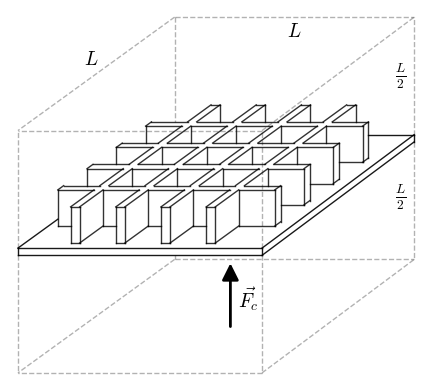
\includegraphics[width=0.48\textwidth]{honeycomb_box_L.png}
\caption{}{Кубическая полость с пластиной \\ покрытой сотами}
\end{center}
\label{fig:honeycomb_box_L}
\end{wrapfigure}

    \section{Двумерный подход
Казимира}\label{ux434ux432ux443ux43cux435ux440ux43dux44bux439-ux43fux43eux434ux445ux43eux434-ux43aux430ux437ux438ux43cux438ux440ux430}

    Рассмотрим кубическую полость объемом \(L^3\), ограниченную идеально
проводящими стенками, и пусть в эту полость параллельно грани \(xy\)
помещена идеально проводящая квадратная пластина со стороной \(L\), и
представим ситуацию, когда эта пластина находится на очень большом,
скажем, \(L/2\) расстоянии a от грани \(xy\).

Одна сторона этой идеально проводящей квадратной пластины представляет
собой чистую плоскость, а другая покрыта идеально проводящими сотами
квадратной формы со стороной квадрата \(a\).

По обеим сторонам пластины выражения \(\sum\hbar\omega\big/2\), где
суммирование распространяется на все возможные резонансные частоты
полости \(L/2\times L\times L\) (большая полость: между чистой
плоскостью и гранью \(xy\)) и полости \(L/2\times a\times a\) (маленькая
полость, одна сотовая ячейка: между донышком сотовой ячейки и
противоположной гранью \(xy\)) расходятся и лишены физического смысла,
но разность этих сумм по противоположные стороны
\(\left(\sum\,\,\hbar\omega\right)_{I}\big/{\left(2\,V_{ I}\right)} - \left(\sum\,\,\hbar\omega\right)_{II}\big/{\left(2\,V_{II}\right)}\),
будет иметь хорошо определенное значение, и это значение будет
интерпретироваться как взаимодействие между пластиной и обеими
удаленными гранями \(xy\).

    Возможные колебания внутри полостей, определяемые

    \(0<=x<=L\), \(0<=y<=L\), \(0<=z<=L/2\) (большая полость: между чистой
плоскостью и гранью \(xy\))

    и

    \(0<=x<=a\), \(0<=y<=a\), \(0<=z<=L/2\) (маленькая полость, одна сотовая
ячейка)

    имеют волновые векторы

    \(k_x = \frac{\pi}{L}\,n_x\), \(k_y = \frac{\pi}{L}\,n_y\),
\(k_z = \frac{\pi}{L/2}\,n_z\) (большая полость: между чистой плоскостью
и гранью \(xy\)),

    и

    \(k_x = \frac{\pi}{a}\,n_x\), \(k_y = \frac{\pi}{a}\,n_y\),
\(k_z = \frac{\pi}{L/2}\,n_z\) (маленькая полость, одна сотовая ячейка),

где \(n_x\). \(n_y\), \(n_z\) положительные целые числа;

    \(k = \sqrt{k_x^2+k_y^2+k_z^2} = \sqrt{\kappa^2+k_z^2}\).

    \(E = \frac{1}{2}\sum\,\hbar\omega = \hbar\,c\frac{1}{2}\sum\limits_{n_x}^{}\sum\limits_{n_y}^{}\sum\limits_{n_z}^{}k\)

    Каждому \(k_x\), \(k_y\), \(k_z\) соответствуют две стоячие волны, если
только одна из \(n_i\) не равна нулю, когда существует только одна.

    В случае маленькой полости для одной сотовой ячейки при очень больших
\(L/2\) мы можем рассматривать \(k_z\) как непрерывную переменную,
заменив суммирование по \(n_z\) на интегрирование. Таким образом, мы
находим

    \(\frac{1}{2}\sum\,\hbar\omega = \hbar\,c\frac{1}{2}\int\limits_{0}^{\infty}\left[{\sqrt{k_z^2}+2\sum\limits_{n_x=1}^{\infty}\sum\limits_{n_y=1}^{\infty}\sqrt{n_x^2\frac{\pi^2}{a^2}+n_y^2\frac{\pi^2}{a^2}+k_z^2}}\right]d{n_z}\)
(маленькая полость, одна сотовая ячейка),

    \(dn_z = \frac{L/2}{\pi}\,dk_z\),

    Теперь мы можем найти удельную плотность энергии \(E/V\), где
\(V = V_{small} = a^2 L/2\):

    \(\frac{1}{2\,V}\sum\,\hbar\omega = \frac{\hbar\,c}{a^2\,L/2}\frac{1}{2}\int\limits_{0}^{\infty}\left[{\sqrt{k_z^2}+2\sum\limits_{n_x=1}^{\infty}\sum\limits_{n_y=1}^{\infty}\sqrt{n_x^2\frac{\pi^2}{a^2}+n_y^2\frac{\pi^2}{a^2}+k_z^2}}\right]\frac{L/2}{\pi}\,dk_z\)
(маленькая полость, одна сотовая ячейка),

    \(\frac{1}{2\,V}\sum\,\hbar\omega = \frac{\hbar\,c}{a^2\,\pi}\int\limits_{0}^{\infty}\left[{\frac{1}{2}\sqrt{k_z^2}+\sum\limits_{n_x=1}^{\infty}\sum\limits_{n_y=1}^{\infty}\sqrt{n_x^2\frac{\pi^2}{a^2}+n_y^2\frac{\pi^2}{a^2}+k_z^2}}\right]\,dk_z\)
(маленькая полость, одна сотовая ячейка),

    \(\frac{1}{2\,V}\sum\,\hbar\omega = \frac{\hbar\,c}{a^2\,\pi}\int\limits_{0}^{\infty}\left[{\sum\limits_{n_x=(0)1}^{\infty}\sum\limits_{n_y=(0)1}^{\infty}\sqrt{n_x^2\frac{\pi^2}{a^2}+n_y^2\frac{\pi^2}{a^2}+k_z^2}}\right]\,dk_z\)
(маленькая полость, одна сотовая ячейка),

    где обозначение \(\left(0\right) 1\) означает, что терм с \(n_x = 0\) и
\(n_y = 0\) должен быть умножен на \(1\big/2\).

    \(\frac{1}{2\,V}\sum\,\hbar\omega = \frac{\hbar\,c}{a^2\,\pi}\sum\limits_{n_x=(0)1}^{\infty}\sum\limits_{n_y=(0)1}^{\infty}\left[\int\limits_{0}^{\infty}\sqrt{n_x^2\frac{\pi^2}{a^2}+n_y^2\frac{\pi^2}{a^2}+k_z^2}\,dk_z\right]\)
(маленькая полость, одна сотовая ячейка),

    И в случае большой полости при очень больших \(L\) мы можем
рассматривать \(k_x\), \(k_y\) как непрерывные переменные. Таким
образом, мы находим

    \(\frac{1}{2}\sum\,\hbar\omega = \hbar\,c\frac{1}{2}\int\limits_{0}^{\infty}\int\limits_{0}^{\infty}\left[{\sqrt{k_x^2+k_y^2}+2\sum\limits_{n_z=1}^{\infty}\sqrt{n_z^2\frac{\pi^2}{(L/2)^2}+k_x^2+k_y^2}}\right]d{n_x}d{n_y}\)
(большая полость: между чистой плоскостью и гранью \(xy\)),

    Для очень больших \(L/2\) и это последнее суммирование можно заменить
интегралом, и поэтому легко видеть, что энергия определяется выражением

    \(\frac{1}{2}\sum\,\hbar\omega = \hbar\,c\int\limits_{0}^{\infty}\int\limits_{0}^{\infty}\int\limits_{0}^{\infty}\sqrt{k_z^2+k_x^2+k_y^2}\,d{n_x}\,d{n_y}\,d{n_z}\)
(большая полость: между чистой плоскостью и гранью \(xy\)),

    \(dn_x = \frac{L}{\pi}\,dk_x\), \(dn_y = \frac{L}{\pi}\,dk_y\),
\(dn_z = \frac{L/2}{\pi}\,dk_z\),

    Теперь мы можем найти удельную плотность энергии \(E/V\), где
\(V = V_{large} = L^3/2\) :

    \(\frac{1}{2\,V}\sum\,\hbar\omega = \frac{\hbar\,c}{L^3/2}\int\limits_{0}^{\infty}\int\limits_{0}^{\infty}\int\limits_{0}^{\infty}\sqrt{k_z^2+k_x^2+k_y^2}\,dn_x\,dn_y\,\frac{L/2}{\pi}\,dk_z\)
(большая полость: между чистой плоскостью и гранью \(xy\)),

    \(\frac{1}{2\,V}\sum\,\hbar\omega = \frac{\hbar\,c}{L^2\,\pi}\int\limits_{0}^{\infty}\int\limits_{0}^{\infty}\left[\,\int\limits_{0}^{\infty}\sqrt{k_z^2+k_x^2+k_y^2}\,dk_z\right]\,dn_x\,dn_y\)
(большая полость: между чистой плоскостью и гранью \(xy\)),

    \(\frac{1}{2\,V}\sum\,\hbar\omega = \frac{\hbar\,c}{L^2\,\pi}\int\limits_{0}^{\infty}\int\limits_{0}^{\infty}\left[\,\int\limits_{0}^{\infty}\sqrt{k_x^2+k_y^2+k_z^2}\,dk_z\right]\,dn_x\,dn_y\)
(большая полость: между чистой плоскостью и гранью \(xy\)),

    \(\frac{1}{2\,V}\sum\,\hbar\omega = \frac{\hbar\,c}{L^2\,\pi}\int\limits_{0}^{\infty}\int\limits_{0}^{\infty}\left[\,\int\limits_{0}^{\infty}\sqrt{k_x^2+k_y^2+k_z^2}\,dk_z\right]\,\left(\frac{L}{\pi}dk_x\right)\,\left(\frac{L}{\pi}dk_y\right)\)
(большая полость: между чистой плоскостью и гранью \(xy\)),

    \(\frac{1}{2\,V}\sum\,\hbar\omega = \frac{\hbar\,c}{a^2\,\pi}\int\limits_{0}^{\infty}\int\limits_{0}^{\infty}\left[\,\int\limits_{0}^{\infty}\sqrt{k_x^2+k_y^2+k_z^2}\,dk_z\right]\,\left(\frac{a}{\pi}dk_x\right)\,\left(\frac{a}{\pi}dk_y\right)\)
(большая полость: между чистой плоскостью и гранью \(xy\)),

    \(\frac{1}{2\,V}\sum\,\hbar\omega = \frac{\hbar\,c}{a^2\,\pi}\sum\limits_{n_x=(0)1}^{\infty}\sum\limits_{n_y=(0)1}^{\infty}\left[\,\int\limits_{0}^{\infty}\sqrt{n_x^2\frac{\pi^2}{a^2}+n_y^2\frac{\pi^2}{a^2}+k_z^2}\,dk_z\right]\)
(маленькая полость, одна сотовая ячейка),

    легко видеть, что наша энергия взаимодействия определяется выражением

    \[\begin{array}{lr}
\delta\,\frac{E}{V} = 
\begin{array}{c}
\frac{\hbar\,c}{a^2\,\pi}\Bigg\{\sum\limits_{n_x=(0)1}^{\infty}\sum\limits_{n_y=(0)1}^{\infty}\left[\,\int\limits_{0}^{\infty}\sqrt{n_x^2\frac{\pi^2}{a^2}+n_y^2\frac{\pi^2}{a^2}+k_z^2}\,dk_z\right] - \\
\int\limits_{0}^{\infty}\int\limits_{0}^{\infty}\left[\,\int\limits_{0}^{\infty}\sqrt{k_x^2+k_y^2+k_z^2}\,dk_z\right]\,\left(\frac{a}{\pi}dk_x\right)\,\left(\frac{a}{\pi}dk_y\right)\Bigg\}
\end{array}\end{array}\]

    \[\begin{array}{lr}
\delta\,\frac{E}{V} =
\begin{array}{c}
\frac{\hbar\,c}{a^2\,\pi}\Bigg\{\sum\limits_{n_x=(0)1}^{\infty}\sum\limits_{n_y=(0)1}^{\infty}\left[\,\int\limits_{0}^{\infty}\sqrt{n_x^2\frac{\pi^2}{a^2}+n_y^2\frac{\pi^2}{a^2}+k_z^2}\,dk_z\right] - \\ \int\limits_{0}^{\infty}\int\limits_{0}^{\infty}\left[\,\int\limits_{0}^{\infty}\sqrt{k_x^2+k_y^2+k_z^2}\,dk_z\right]\,dn_x\,dn_y\Bigg\}
\end{array}\end{array}\]

    

    \({\left(\frac{E}{V}\right)_{small\,cavity} = \frac{1}{a^2}\,\hbar \, \sum\limits_{n_x=(0)1}^{\infty}\sum\limits_{n_y=(0)1}^{\infty}\,\int\limits_{0}^{\infty} {\frac {dk_{z}}{\pi}}\,\omega _{n_x,n_y},}\)

    где
\(\omega _{n_x,n_y} = c\,\sqrt{n_x^2\frac{\pi^2}{a^2}+n_y^2\frac{\pi^2}{a^2}+k_z^2}\)

    Очевидно, что это выражение бесконечно, и чтобы продолжить расчет,
удобно ввести регулятор.

    Для получения конечного результата необходимо умножить подынтегральные
выражения на регуляризационную функцию \(f(k/k_m)\), которая равна
единице при \(k << k_m\), но достаточно быстро стремится к нулю при
\((k/k_m)\, \rightarrow\,\infty\). Где \(k_m\) можно определить как
\(f(1) = \frac{1}{2}\). Физический смысл очевиден: для очень коротких
волн (например, рентгеновских лучей) наша пластина вообще не является
препятствием, и поэтому на энергию нулевой точки этих волн не будет
влиять положение этой пластины.

    Функция регуляризации будет служить для того, чтобы сделать выражение
конечным, и в конце концов влияние ее конкретного вида устраняется
предельным переходом.

    Вводя переменную \(u^2 = a^2\,k_z^2/\pi^2\), \(du = a/\pi\,dk_z\),
имеем:

    \begin{equation}
\begin{array}{lr}
\delta\,\frac{E}{V} =
\begin{array}{c}
\frac{\hbar\,c\,\pi}{a^4}\Bigg\{
\sum\limits_{n_x=\left(0\right)\,1}^{\infty}
\sum\limits_{n_y=\left(0\right)\,1}^{\infty}
\int\limits_{0}^{\infty}
{\sqrt{n_x^2 + n_y^2 + u^2}}
f\left(\frac{\pi\sqrt{n_x^2 + n_y^2 + u^2}}{a\,k_m}\right)
\,d{u} \\
- \int\limits_{0}^{\infty}
\int\limits_{0}^{\infty}
\int\limits_{0}^{\infty}
{\sqrt{n_x^2 + n_y^2 + u^2}}
f\left(\frac{\pi\sqrt{n_x^2 + n_y^2 + u^2}}{a\,k_m}\right)
\,d{u}\,d{n_x}\,d{n_y}
\Bigg\}
\end{array}
\end{array}
\end{equation}

    If
\(\omega _{n_x,n_y} = c\,\sqrt{n_x^2\frac{\pi^2}{a^2}+n_y^2\frac{\pi^2}{a^2}+k_z^2}\)
и \(k_z^2 = u^2 \frac{\pi^2}{a^2}\) имеем
\(\omega _{n_x,n_y} = c \, \frac{\pi}{a} \sqrt{n_x^2+n_y^2+u^2}\) so
\(f\left(\frac{\pi\sqrt{n_x^2 + n_y^2+u^2}}{a\,k_m}\right) = f\left(\frac{\omega _{n_x,n_y}}{c\,k_m}\right)\)
где частота обрезания \(\omega_m = c\,k_m\)

    Путем введения функции:

    \begin{equation}
F\left(u, n_x, n_y\right) = 
\sqrt{n_x^2 + n_y^2+u^2}\,
f\left(\frac{\pi\sqrt{n_x^2 + n_y^2+u^2}}{a\,k_m}\right)
\end{equation}

    мы можем записать:

    \begin{equation}
\begin{array}{lr}
\delta\,\frac{E}{V} =
\begin{array}{c}
\frac{\hbar\,c\,\pi}{a^4}
\Bigg\{
\sum\limits_{n_x=\left(0\right)\,1}^{\infty}
\sum\limits_{n_y=\left(0\right)\,1}^{\infty}
\left(\int\limits_{0}^{\infty}F\left(u, n_x, n_y\right)\,d{u}\right)
- \\
\int\limits_{0}^{\infty}
\int\limits_{0}^{\infty}
\left(\int\limits_{0}^{\infty}F\left(u, n_x, n_y\right)\,d{u}\right)
\,d{n_x}\,d{n_y}
\Bigg\}
\end{array}
\end{array}
\end{equation}

    И наконец, используя

    \begin{equation}
G\left(n_x, n_y\right) = \int\limits_{0}^{\infty}F\left(u, n_x, n_y\right)\,d{u}
\end{equation}

    Имеем

    \begin{equation}
\delta\,\frac{E}{V} = \frac{\hbar\,c\,\pi}{a^4}
\left\{
\sum\limits_{n_x=\left(0\right)\,1}^{\infty}
\sum\limits_{n_y=\left(0\right)\,1}^{\infty}
G\left(n_x, n_y\right)
-
\int\limits_{0}^{\infty}
\int\limits_{0}^{\infty}
G\left(n_x, n_y\right)
\,d{n_x}\,d{n_y}
\right\}
\end{equation}

Интегрирование функции \(G\left(n_x, n_y\right)\) с тестовой функцией
регуляризации см. в Приложении A.

    Теперь, стремясь получить способ вычисления \(\delta\left(E/V\right)\),
мы должны рассмотреть

\section{Двумерную формулу Эйлера --
Маклорена}\label{ux434ux432ux443ux43cux435ux440ux43dux443ux44e-ux444ux43eux440ux43cux443ux43bux443-ux44dux439ux43bux435ux440ux430-ux43cux430ux43aux43bux43eux440ux435ux43dux430}

В соответствии с A.Bikyalis \cite{Bikyalis1968} мы просто дважды
применяем формулу Эйлера - Маклорена к \(n_x\) и к \(n_y\)

Начиная со следующего представления этой формулы

\[{\displaystyle \sum _{i=a}^{b}f(i)=\int _{a}^{b}f(x)\,dx+{\frac {f(a)+f(b)}{2}}+\sum _{k=1}^{\lfloor p/2\rfloor }{\frac {B_{2k}}{(2k)!}}\left(f^{(2k-1)}(b)-f^{(2k-1)}(a)\right)+R_{p},}\]

\[{\displaystyle P_{k}(x)=B_{k}\left(x-\lfloor x\rfloor \right),}\]

\[{\displaystyle R_{p}=(-1)^{p+1}\int _{a}^{b}f^{(p)}(x){\frac {P_{p}(x)}{p!}}\,dx.}\]

или лучше поскольку мы имеем дело с математически весьма сложной задачей
численного интегрирования довольно непростой, часто осциллирующей и
терпящей разрывы в точках каждого целого значения аргумента благодаря
наличию множителя \((x-\lfloor x\rfloor )\) функции, воспользуемся тем,
что остаточный член можно выразить также в виде:

\[{\displaystyle R_{p}=(-1)^{p+1}\sum_{j=a}^{b-1} \int _{0}^{1}f^{(p)}(v+j){\frac {B_{p}(v)}{p!}}\,dv.}\]

мы видим, что она состоит из 4 членов:

интеграл \(\int\limits_{x}^{}=\int _{x_a}^{x_b}f(x)\,dx\),

половинная сумма
\(\underset{x}{H_{\sum}}={\left( {f(x_a)+f(x_b)}\right)/{2}}\),

сумма многочленов Бернулли
\({\sum\limits_{x}^{}}^{B}=\sum _{k=1}^{\lfloor p/2\rfloor }{\frac {B_{2k}}{(2k)!}}\left(f^{(2k-1)}(x_b)-f^{(2k-1)}(x_a)\right)\)

и остаточный член
\(\underset{x}{R_{p}}=(-1)^{p+1}\sum_{j=x_a}^{x_b-1} \int _{0}^{1}f^{(p)}(v_x+j_x){\frac {B_{p}(v_x)}{p!}}\,dv_x\).

Применяя её дважды к \(G\) по \(n_x\) и по \(n_y\), мы получим следующие
термы, которые можно представить в виде таблицы:

    \begin{equation}
\begin{array}{cccc}
 \int\limits_{n_y}^{} \int\limits_{n_x}^{} G  &  \int\limits_{n_y}^{} \underset{n_x}{H_{\sum}}\,G  &  \int\limits_{n_y}^{}{\sum\limits_{n_x}^{}}^{B}\,G  &  \int\limits_{n_y}^{}\,\underset{n_x}{R_{p}}\,G  \\
 \underset{n_y}{H_{\sum}}\,\int\limits_{n_x}^{}\,G &  \underset{n_y}{H_{\sum}}\,\underset{n_x}{H_{\sum}}\,G &  \underset{n_y}{H_{\sum}}\,{\sum\limits_{n_x}^{}}^{B}\,G &  \underset{n_y}{H_{\sum}}\,\underset{n_x}{R_{p}}\,G \\
 {\sum\limits_{n_y}^{}}^{B}\,\int\limits_{n_x}^{}\,G  &  {\sum\limits_{n_y}^{}}^{B}\,\underset{n_x}{H_{\sum}}\,G  &  {\sum\limits_{n_y}^{}}^{B}\,{\sum\limits_{n_x}^{}}^{B}\,G  &  {\sum\limits_{n_y}^{}}^{B}\,\underset{n_x}{R_{p}}\,G  \\
 \underset{n_y}{R_{p}}\,\int\limits_{n_x}^{}\,G   &  \underset{n_y}{R_{p}}\,\underset{n_x}{H_{\sum}}\,G   &  \underset{n_y}{R_{p}}\,{\sum\limits_{n_x}^{}}^{B}\,G   &  \underset{n_y}{R_{p}}\,\underset{n_x}{R_{p}}\,G
\end{array}\end{equation}

    А учитывая, что у нас есть функция \(G\), симметричная относительно
своих аргументов \(n_x\) и \(n_y\), значит, приведенная выше двумерная
матрица Эйлера--Маклорена тоже симметрична.

    \section{Сводка двумерного Эйлера --
Маклорена}\label{ux441ux432ux43eux434ux43aux430-ux434ux432ux443ux43cux435ux440ux43dux43eux433ux43e-ux44dux439ux43bux435ux440ux430-ux43cux430ux43aux43bux43eux440ux435ux43dux430}

Принимая значение параметра \(p = 1\), имеем:

    \begin{center}
\begin{tabular}{ | l | }
\hline

$\int\limits_{n_y}^{} \int\limits_{n_x}^{} G = \int_{a_{y}}^{b_{y}} \int_{a_{x}}^{b_{x}} G\left(n_{x}, n_{y}\right)\,{d n_{x}}\,{d n_{y}}$ \\

$\int\limits_{n_y}^{} \underset{n_x}{H_{\sum}}\,G = \frac{1}{2} \, \int_{a_{y}}^{b_{y}} G\left(a_{x}, n_{y}\right)\,{d n_{y}}$ \\

$\int\limits_{n_y}^{} {\sum\limits_{n_x}^{}}^{B}\,G = 0$ \\

$\int\limits_{n_y}^{} \underset{n_x}{R_{p}}\,G = {\sum_{j_{x}=a_{x}}^{b_{x} - 1} \int_{a_{y}}^{b_{y}} \int_{0}^{1} \frac{1}{2} \, {\left(2 \, v_{n_{x}} - 1\right)} \mathrm{D}_{0}\left(G\right)\left(j_{x} + v_{n_{x}}, n_{y}\right)\,{d v_{n_{x}}}\,{d n_{y}}}$ \\

\hline\hline

$\underset{n_y}{H_{\sum}}\,\int\limits_{n_x}^{}\,G = \frac{1}{2} \, \int_{a_{x}}^{b_{x}} G\left(n_{x}, a_{y}\right)\,{d n_{x}}$ \\

$\underset{n_y}{H_{\sum}}\,\underset{n_x}{H_{\sum}}\,G = \frac{1}{4} \, G\left(a_{x}, a_{y}\right)$ \\

$\underset{n_y}{H_{\sum}}\,{\sum\limits_{n_x}^{}}^{B}\,G = 0$ \\

$\underset{n_y}{H_{\sum}}\,\underset{n_x}{R_{p}}\,G = {\sum_{j_{n_{x}}=a_{x}}^{b_{x} - 1} \frac{1}{4} \, \int_{0}^{1} \left(2 \, v_{n_{x}} - 1 \right) \mathrm{D}_{0}\left(G\right)\left(j_{n_{x}} + v_{n_{x}}, a_{y}\right)\,{d v_{n_{x}}} }$ \\

\hline\hline

${\sum\limits_{n_y}^{}}^{B}\,\int\limits_{n_x}^{}\,G = 0$ \\

${\sum\limits_{n_y}^{}}^{B}\,\underset{n_x}{H_{\sum}}\,G = 0$ \\

${\sum\limits_{n_y}^{}}^{B}\,{\sum\limits_{n_x}^{}}^{B}\,G = 0$ \\

${\sum\limits_{n_y}^{}}^{B}\,\underset{n_x}{R_{p}}\,G = 0$ \\

\hline\hline

$\underset{n_y}{R_{p}}\,\int\limits_{n_x}^{}\,G = {\sum_{j_{x}=a_{x}}^{b_{x} - 1} \int_{a_{y}}^{b_{y}} \int_{0}^{1} \frac{1}{2} \, {\left(2 \, v_{n_{x}} - 1\right)} \mathrm{D}_{0}\left(G\right)\left(j_{x} + v_{n_{x}}, n_{y}\right)\,{d v_{n_{x}}}\,{d n_{y}}}$ \\

$\underset{n_y}{R_{p}}\,\underset{n_x}{H_{\sum}}\,G = {\sum_{j_{n_{y}}=a_{y}}^{b_{y} - 1} \int_{0}^{1} \frac{1}{4} \, {\left(2 \, v_{n_{y}} - 1\right)} \mathrm{D}_{1}\left(G\right)\left(a_{x}, j_{n_{y}} + v_{n_{y}}\right)\,{d v_{n_{y}}}}$ \\

$\underset{n_y}{R_{p}}\,{\sum\limits_{n_x}^{}}^{B}\,G = 0$ \\

$\underset{n_y}{R_{p}}\,\underset{n_x}{R_{p}}\,G = {\sum_{j_{y}=a_{y}}^{b_{y} - 1} {\sum_{j_{x}=a_{x}}^{b_{x} - 1} \int_{0}^{1} \int_{0}^{1}\frac{1}{4} \, {\left(2 \, v_{y} - 1\right)}  {\left(2 \, v_{x} - 1\right)} \mathrm{D}_{0, 1}\left(G\right)\left(j_{x} + v_{x}, j_{y} + v_{y}\right)\,{d v_{x}}}\,{d v_{y}}}$ \\

\hline

\end{tabular}
\end{center}

    \section{\texorpdfstring{Способ расчета
\(\delta\left(E/V\right)\)}{Способ расчета \textbackslash{}delta\textbackslash{}left(E/V\textbackslash{}right)}}\label{ux441ux43fux43eux441ux43eux431-ux440ux430ux441ux447ux435ux442ux430-deltaleftevright}

    Давайте рассмотрим

\[
\sum\limits_{n_x=\left(0\right)\,1}^{\infty}
\sum\limits_{n_y=\left(0\right)\,1}^{\infty}
G\left(n_x, n_y\right)
-
\int\limits_{0}^{\infty}
\int\limits_{0}^{\infty}
G\left(n_x, n_y\right)\,d{n_x}\,d{n_y}
\]

    Сначала мы видим, что

    \(\sum\limits_{n_x=\left(0\right)\,1}^{\infty} \sum\limits_{n_y=\left(0\right)\,1}^{\infty} {G\left(n_x, n_y\right)} = \\ \sum\limits_{n_x=\left(0\right)\,1}^{\infty} \left( -\frac{1}{2}G\left(n_x, 0\right) + \sum\limits_{n_y=0}^{\infty}{G\left(n_x, n_y\right)} \right) = \\ -\frac{1}{2} \left( -\frac{1}{2}G\left(0, 0\right) + \sum\limits_{n_y=0}^{\infty}{G\left(0, n_y\right)} \right) +\sum\limits_{n_x=0}^{\infty} \left( -\frac{1}{2}G\left(n_x, 0\right) + \sum\limits_{n_y=0}^{\infty}{G\left(n_x, n_y\right)} \right) = \\ \frac{1}{4}G\left(0, 0\right) - \frac{1}{2}\sum\limits_{n_y=0}^{\infty}{G\left(0, n_y\right)} - \frac{1}{2}\sum\limits_{n_x=0}^{\infty}{G\left(n_x, 0\right)} + \sum\limits_{n_x=0}^{\infty}\sum\limits_{n_y=0}^{\infty}{G\left(n_x, n_y\right)}\)

    Итак, мы имеем

\(\sum\limits_{n_x=\left(0\right)\,1}^{\infty} \sum\limits_{n_y=\left(0\right)\,1}^{\infty} G\left(n_x, n_y\right) - \int\limits_{0}^{\infty} \int\limits_{0}^{\infty} G\left(n_x, n_y\right)\,d{n_x}\,d{n_y} = \\ \frac{1}{4}G\left(0, 0\right) -\frac{1}{2}\sum\limits_{n_y=0}^{\infty}{G\left(0, n_y\right)} -\frac{1}{2}\sum\limits_{n_x=0}^{\infty}{G\left(n_x, 0\right)} +\sum\limits_{n_x=0}^{\infty}\sum\limits_{n_y=0}^{\infty}{G\left(n_x, n_y\right)} - \int\limits_{0}^{\infty} \int\limits_{0}^{\infty} G\left(n_x, n_y\right)\,d{n_x}\,d{n_y}\)

    С другой стороны, мы обнаружили, что

\(\sum\limits_{n_x=0}^{\infty} \sum\limits_{n_y=0}^{\infty} G\left(n_x, n_y\right) -\int\limits_{0}^{\infty} \int\limits_{0}^{\infty} G\left(n_x, n_y\right)\,d{n_x}\,d{n_y} = \\ \begin{array}{cccc}  \, &  \int\limits_{n_y}^{} \underset{n_x}{H_{\sum}}\,G &  + \int\limits_{n_y}^{}{\sum\limits_{n_x}^{}}^{B}\,G &  + \int\limits_{n_y}^{}\,\underset{n_x}{R_{p}}\,G \\  +\underset{n_y}{H_{\sum}}\,\int\limits_{n_x}^{}\,G &  + \underset{n_y}{H_{\sum}}\,\underset{n_x}{H_{\sum}}\,G &  + \underset{n_y}{H_{\sum}}\,{\sum\limits_{n_x}^{}}^{B}\,G &  + \underset{n_y}{H_{\sum}}\,\underset{n_x}{R_{p}}\,G \\  + {\sum\limits_{n_y}^{}}^{B}\,\int\limits_{n_x}^{}\,G &  + {\sum\limits_{n_y}^{}}^{B}\,\underset{n_x}{H_{\sum}}\,G &  + {\sum\limits_{n_y}^{}}^{B}\,{\sum\limits_{n_x}^{}}^{B}\,G &  + {\sum\limits_{n_y}^{}}^{B}\,\underset{n_x}{R_{p}}\,G \\  + \underset{n_y}{R_{p}}\,\int\limits_{n_x}^{}\,G &  + \underset{n_y}{R_{p}}\,\underset{n_x}{H_{\sum}}\,G &  + \underset{n_y}{R_{p}}\,{\sum\limits_{n_x}^{}}^{B}\,G &  + \underset{n_y}{R_{p}}\,\underset{n_x}{R_{p}}\,G \end{array}\)

    где \(\underset{n_y}{H_{\sum}}\,\underset{n_x}{H_{\sum}}\,G\),
\(\int\limits_{n_y}^{} \underset{n_x}{H_{\sum}}\,G\) и
\(\underset{n_y}{H_{\sum}}\,\int\limits_{n_x}^{}\,G\) есть
соответственно:

    \(\frac{1}{4} \, G\left(a_{x}, a_{y}\right) , \frac{1}{2} \, \int_{a_{y}}^{b_{y}} G\left(a_{x}, n_{y}\right)\,{d n_{y}} , \frac{1}{2} \, \int_{a_{x}}^{b_{x}} G\left(n_{x}, a_{y}\right)\,{d n_{x}}\)

    Теперь, используя одномерную формулу Эйлера-Маклорена в виде:

    \[{\displaystyle \sum _{i=a}^{b}f(i)=\int _{a}^{b}f(x)\,dx+{\frac {f(a)+f(b)}{2}}+\sum _{k=1}^{\lfloor p/2\rfloor }{\frac {B_{2k}}{(2k)!}}(f^{(2k-1)}(b)-f^{(2k-1)}(a))+R_{p},}\]

    мы видим, что

    \[
\frac{1}{4}G\left(0, 0\right)
- \frac{1}{2}\sum\limits_{n_y=0}^{\infty}{G\left(0, n_y\right)}
- \frac{1}{2}\sum\limits_{n_x=0}^{\infty}{G\left(n_x, 0\right)}
\]

    будет равно

    \(\begin{array}{rrllll}  \underset{n_y}{H_{\sum}}\,\underset{n_x}{H_{\sum}}\,G \\  \, &  - \int\limits_{n_y}^{} \underset{n_x}{H_{\sum}}\,G &  - \underset{n_y}{H_{\sum}} \underset{n_x}{H_{\sum}}\,G &  - \frac{1}{2}{\sum\limits_{n_y}^{}}^{B}\,G &  - \frac{1}{2}\underset{n_y}{R_{p}}\,G/2 \\  \,&  - \underset{n_y}{H_{\sum}}\int\limits_{n_x}^{} \,G &  - \underset{n_y}{H_{\sum}} \underset{n_x}{H_{\sum}}\,G &  - \frac{1}{2}{\sum\limits_{n_x}^{}}^{B}\,G &  - \frac{1}{2}\underset{n_x}{R_{p}}\,G/2 \\ \end{array}\)

    Итак, мы можем найти

\(\sum\limits_{n_x=\left(0\right)\,1}^{\infty} \sum\limits_{n_y=\left(0\right)\,1}^{\infty} G\left(n_x, n_y\right) - \int\limits_{0}^{\infty} \int\limits_{0}^{\infty} G\left(n_x, n_y\right)\,d{n_x}\,d{n_y}\)

используя следующую формулу:

    \(\begin{array}{llll}  \,&  \,&  + \int\limits_{n_y}^{}{\sum\limits_{n_x}^{}}^{B}\,G &  + \int\limits_{n_y}^{}\,\underset{n_x}{R_{p}}\,G \\  \,&  \,&  + \underset{n_y}{H_{\sum}}\,{\sum\limits_{n_x}^{}}^{B}\,G &  + \underset{n_y}{H_{\sum}}\,\underset{n_x}{R_{p}}\,G \\  + {\sum\limits_{n_y}^{}}^{B}\,\int\limits_{n_x}^{}\,G &  + {\sum\limits_{n_y}^{}}^{B}\,\underset{n_x}{H_{\sum}}\,G &  + {\sum\limits_{n_y}^{}}^{B}\,{\sum\limits_{n_x}^{}}^{B}\,G &  + {\sum\limits_{n_y}^{}}^{B}\,\underset{n_x}{R_{p}}\,G \\  + \underset{n_y}{R_{p}}\,\int\limits_{n_x}^{}\,G &  + \underset{n_y}{R_{p}}\,\underset{n_x}{H_{\sum}}\,G &  + \underset{n_y}{R_{p}}\,{\sum\limits_{n_x}^{}}^{B}\,G &  + \underset{n_y}{R_{p}}\,\underset{n_x}{R_{p}}\,G \\  \,&  \,&  - \frac{1}{2}{\sum\limits_{n_y}^{}}^{B}\,G &  - \frac{1}{2}\underset{n_y}{R_{p}}\,G \\  \,&  \,&  - \frac{1}{2}{\sum\limits_{n_x}^{}}^{B}\,G &  - \frac{1}{2}\underset{n_x}{R_{p}}\,G \\ \end{array}\)

    Легко видеть, что все слагаемые без остаточного члена

    \(\begin{array}{llll}  \,&  \,&  + \int\limits_{n_y}^{}{\sum\limits_{n_x}^{}}^{B}\,G \\  \,&  \,&  + \underset{n_y}{H_{\sum}}\,{\sum\limits_{n_x}^{}}^{B}\,G \\  + {\sum\limits_{n_y}^{}}^{B}\,\int\limits_{n_x}^{}\,G &  + {\sum\limits_{n_y}^{}}^{B}\,\underset{n_x}{H_{\sum}}\,G &  + {\sum\limits_{n_y}^{}}^{B}\,{\sum\limits_{n_x}^{}}^{B}\,G\\  \,&  \,&  - \frac{1}{2}{\sum\limits_{n_y}^{}}^{B}\,G \\  \,&  \,&  - \frac{1}{2}{\sum\limits_{n_x}^{}}^{B}\,G \\ \end{array}\)

    в сумме равны 0. И поэтому любой возможный ненулевой результат должен
быть связан с остатком:

    \(\begin{array}{r} \sum\limits_{n_x=\left(0\right)\,1}^{\infty} \sum\limits_{n_y=\left(0\right)\,1}^{\infty} G\left(n_x, n_y\right) - \int\limits_{0}^{\infty} \int\limits_{0}^{\infty} G\left(n_x, n_y\right)\,d{n_x}\,d{n_y} = \end{array}\)

    \(\begin{array}{llll}  \,&  \,&  \,&  + \int\limits_{n_y}^{}\,\underset{n_x}{R_{p}}\,G \\  \,&  \,&  \,&  + \underset{n_y}{H_{\sum}}\,\underset{n_x}{R_{p}}\,G \\  \,&  \,&  \,&  + {\sum\limits_{n_y}^{}}^{B}\,\underset{n_x}{R_{p}}\,G \\  + \underset{n_y}{R_{p}}\,\int\limits_{n_x}^{}\,G &  + \underset{n_y}{R_{p}}\,\underset{n_x}{H_{\sum}}\,G &  + \underset{n_y}{R_{p}}\,{\sum\limits_{n_x}^{}}^{B}\,G &  + \underset{n_y}{R_{p}}\,\underset{n_x}{R_{p}}\,G \\  \,&  \,&  \,&  - \frac{1}{2}\underset{n_y}{R_{p}}\,G \\  \,&  \,&  \,&  - \frac{1}{2}\underset{n_x}{R_{p}}\,G \\ \end{array}\)

    Или, используя симметричные свойства \(G\), мы можем переписать
результирующую формулу:

    \(\begin{array}{r} \sum\limits_{n_x=\left(0\right)\,1}^{\infty} \sum\limits_{n_y=\left(0\right)\,1}^{\infty} G\left(n_x, n_y\right) - \int\limits_{0}^{\infty} \int\limits_{0}^{\infty} G\left(n_x, n_y\right)\,d{n_x}\,d{n_y} = \end{array}\)

    \(+\,2\cdot\underset{n_y}{R_{p}}\,\int\limits_{n_x}^{}\,G +\,2\cdot\underset{n_y}{R_{p}}\,\underset{n_x}{H_{\sum}}\,G +\,2\cdot\underset{n_y}{R_{p}}\,{\sum\limits_{n_x}^{}}^{B}\,G +\,\underset{n_y}{R_{p}}\,\underset{n_x}{R_{p}}\,G -\,\underset{n_y}{R_{p}}\,G\)

    со следующими слагаемыми:

\(2\cdot\underset{n_y}{R_{p}}\,\int\limits_{n_x}^{}\,G\left(u\right) = 2 \, {\sum\limits_{j_{x}=a_{x}}^{b_{x} - 1} \int\limits_{a_{y}}^{b_{y}} \int\limits_{0}^{1} \frac{1}{2} \, {\left(2 \, v_{n_{x}} - 1\right)} \mathrm{D}_{0}\left(G\right)\left(j_{x} + v_{n_{x}}, n_{y}\right)\,{d v_{n_{x}}}\,{d n_{y}}}\)

\(2\cdot\underset{n_y}{R_{p}}\,\underset{n_x}{H_{\sum}}\,G\left(u\right) = 2 \, {\sum\limits_{j_{n_{y}}=a_{y}}^{b_{y} - 1} \int\limits_{0}^{1} \frac{1}{4} \, {\left(2 \, v_{n_{y}} - 1\right)} \mathrm{D}_{1}\left(G\right)\left(a_{x}, j_{n_{y}} + v_{n_{y}}\right)\,{d v_{n_{y}}}}\)

\(2\cdot\underset{n_y}{R_{p}}\,{\sum\limits_{n_x}^{}}^{B}\,G\left(u\right) = 2 \, {\sum\limits_{j_{n_{y}}=a_{y}}^{b_{y} - 1} \int\limits_{0}^{1} 0\,{d v_{n_{y}}}}\)

\(\underset{n_y}{R_{p}}\,\underset{n_x}{R_{p}}\,G = {\sum\limits_{j_{y}=a_{y}}^{b_{y} - 1} {\sum\limits_{j_{x}=a_{x}}^{b_{x} - 1} \int\limits_{0}^{1} \int\limits_{0}^{1} \frac{1}{4} \, {\left(2 \, v_{y} - 1\right)} {\left(2 \, v_{x} - 1\right)} \mathrm{D}_{0, 1}\left(G\right)\left(j_{x} + v_{x}, j_{y} + v_{y}\right)\,{d v_{x}}}\,{d v_{y}}}\)

\(-\underset{n_y}{R_{p}}\,G = -{\sum\limits_{j_{n_{y}}=a_{y}}^{b_{y} - 1} \int\limits_{0}^{1} \frac{1}{2} \, {\left(2 \, v_{n_{y}} - 1\right)} \mathrm{D}_{1}\left(G\right)\left(n_{x}, j_{n_{y}} + v_{n_{y}}\right)\,{d v_{n_{y}}}}\)

    Учитывая, что \(\underset{n_y}{R_{p}}\,{\sum\limits_{n_x}^{}}^{B}\,G\)
должно быть равно \(0\), потому что производная по \(n_x\) при
\(n_x = 0\) дает \(0\), а
\(\,2\cdot\underset{n_y}{R_{p}}\,\underset{n_x}{H_{\sum}}\,G -\,\underset{n_y}{ R_{p}}\,G\)
дает \(0\) в сумме, мы можем упростить результат в виде:

    \begin{equation}
\begin{array}{r}
\sum\limits_{n_x=\left(0\right)\,1}^{\infty}
\sum\limits_{n_y=\left(0\right)\,1}^{\infty}
G\left(n_x, n_y\right)
-
\int\limits_{0}^{\infty}
\int\limits_{0}^{\infty}
G\left(n_x, n_y\right)\,d{n_x}\,d{n_y} =
\,2\cdot\underset{n_y}{R_{p}}\,\int\limits_{n_x}^{}\,G 
+\,\underset{n_y}{R_{p}}\,\underset{n_x}{R_{p}}\,G
\end{array}
\end{equation}

    или в подробной форме:

\begin{equation}
\begin{array}{l}
\sum\limits_{n_x=\left(0\right)\,1}^{\infty}
\sum\limits_{n_y=\left(0\right)\,1}^{\infty}
G\left(n_x, n_y\right)
-
\int\limits_{0}^{\infty}
\int\limits_{0}^{\infty}
G\left(n_x, n_y\right)\,d{n_x}\,d{n_y} = \\
{\sum\limits_{j_{x}=0}^{\infty} \int\limits_{n_{y}=0}^{\infty} \int\limits_{v_x=0}^{1}  {\left(2 \, v_{n_{x}} - 1\right)} \mathrm{D}_{0}\left(G\right)\left(j_{x} + v_{n_{x}}, n_{y}\right)\,{d v_{n_{x}}}\,{d n_{y}}} + \\
\frac{1}{4} \, {\sum\limits_{j_{y}=0}^{\infty} {\sum\limits_{j_{x}=0}^{\infty} \int\limits_{0}^{1} \int\limits_{0}^{1} {\left(2 \, v_{y} - 1\right)} {\left(2 \, v_{x} - 1\right)} \mathrm{D}_{0, 1}\left(G\right)\left(j_{x} + v_{x}, j_{y} + v_{y}\right)\,{d v_{x}}}\,{d v_{y}}}
\end{array}
\end{equation}

    \section{\texorpdfstring{Как \(\delta\left(E/V\right)\) зависит от
\(a k_m\)
?}{Как \textbackslash{}delta\textbackslash{}left(E/V\textbackslash{}right) зависит от a k\_m ?}}\label{ux43aux430ux43a-deltaleftevright-ux437ux430ux432ux438ux441ux438ux442-ux43eux442-a-k_m}

    Казимир в своей оригинальной работе представил свою формулу в
предположении, что \(a\,k_m\,»\,1\). Но теперь мы можем исследовать, как

\(\sum\limits_{n_x=\left(0\right)\,1}^{\infty} \sum\limits_{n_y=\left(0\right)\,1}^{\infty} G\left(n_x, n_y\right) - \int\limits_{0}^{\infty} \int\limits_{0}^{\infty} G\left(n_x, n_y\right)\,d{n_x}\,d{n_y}\)

будет зависеть от \(a k_m\)

    \begin{center}
\begin{tabular}{ | l | c | c | c | }
\hline
$a \cdot k_m$ & $\sum\limits_{\left(0\right)\,1}^{\infty}\sum\limits_{\left(0\right)\,1}^{\infty}-\int\limits_{0}^{\infty}\int\limits_{0}^{\infty}G$ & $\epsilon$ & $j_{max}$ \\
\hline
0.25 & 0.0010898998026781217 & 4.996697073620143e-07 & 2 \\
0.5 & 0.0032237749029524953 & 7.998369526561223e-07 & 6 \\
0.75 & 0.004403922584267899 & 8.721734991096397e-07 & 11 \\
1.0 & 0.003048368039753142 & 8.495559555607291e-07 & 17 \\
1.25 & -0.0014811539004775248 & 1.7711588730298828e-06 & 18 \\
1.5 & -0.008708226320289525 & 3.6727148564415e-06 & 18 \\
1.75 & -0.01722786703218093 & 6.80405403998826e-06 & 18 \\
2.0 & -0.025174603512904688 & 9.989436530283013e-06 & 19 \\
2.25 & -0.030834142522710325 & 9.370330676246764e-06 & 23 \\
2.5 & -0.03328670643720081 & 1.4281938944775391e-05 & 23 \\
2.75 & -0.03243630208049284 & 2.091015549165456e-05 & 23 \\
3.0 & -0.028986396523536337 & 2.961508478431949e-05 & 23 \\
3.25 & -0.024047951283080123 & 4.0789713256873105e-05 & 23 \\
3.5 & -0.018309169743688476 & 8.561178612309775e-06 & 45 \\
3.75 & -0.013591792977477306 & 2.1853680230903085e-05 & 36 \\
4 & -0.009731507224089121 & 1.4610545561998458e-05 & 45 \\
4.5 & -0.006342700310733549 & 1.9329818693328873e-05 & 48 \\
5 & -0.007323343929996339 & 2.3242272627768528e-05 & 52 \\
6 & -0.012436017530558603 & 2.3732800946523056e-05 & 66 \\
7 & -0.014209420986523558 & 3.8533275062919475e-05 & 69 \\
8 & -0.0136610172109347 & 3.293747500025098e-05 & 87 \\
9 & -0.013782731174753638 & 3.585979757156756e-05 & 99 \\
\hline
\end{tabular}
\end{center}

    Таким образом, для разности плотности энергии на \(sm^2\) находим

    \(\delta\,\frac{E}{V} = \frac{\hbar\,c\,\pi}{a^4} \int\limits_{0}^{\infty}{ \left\{ \sum\limits_{n_x=\left(0\right)\,1}^{\infty} \sum\limits_{n_y=\left(0\right)\,1}^{\infty} F\left(n_x, n_y\right) - \int\limits_{0}^{\infty} \int\limits_{0}^{\infty} F\left(n_x, n_y\right)\,d{n_x}\,d{n_y} \right\} }\,d{u}\)

    В соответствии с нашими расчетами мы видим, что

    \(\int\limits_{0}^{\infty}{ \left\{ \sum\limits_{n_x=\left(0\right)\,1}^{\infty} \sum\limits_{n_y=\left(0\right)\,1}^{\infty} F\left(n_x, n_y\right) - \int\limits_{0}^{\infty} \int\limits_{0}^{\infty} F\left(n_x, n_y\right)\,d{n_x}\,d{n_y} \right\} }\,d{u} \approx R\left(a k_m\right)\)

    \begin{wrapfigure}{r}{0.5\textwidth}
\begin{center}
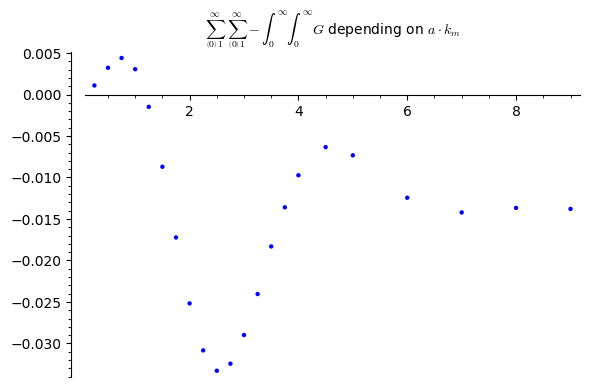
\includegraphics[width=0.48\textwidth]{sum_sum_int_int_G_on_a_km.png}
\caption{}{How $\delta\left(E/V\right)$ depends on $a k_m$}
\end{center}
\label{fig:G_on_a_km}
\end{wrapfigure}

    Где \(R\left(a k_m\right)\) --- некоторая функция, зависящая от свойств
материала, с четко определенным пределом при \(a\,k_m\,»\,1\). Итак,

    \begin{equation}
\delta\,\frac{E}{V} = R\left(a k_m\right)\,\frac{\hbar\,c\,\pi}{a^4}
\end{equation}

    Для разности плотности энергии на \(sm^2\) (в пределе при
\(a\,k_m\,\rightarrow \,10\)) находим

    \(\delta\,\frac{E}{V} = \hbar\,c\, \pi\frac{R}{a^4}\,=\,0.0136\,\frac{1}{a_{\mu}^4}\,dyne/cm^2\)

    где \(a_{\mu}\) --- сторона квадрата сот, измеряемая в микронах.

    Можно ли интерпретировать эту разницу удельной плотности энергии
\(\delta\left(E/V\right)\) как причину действия силы \(F\) на идеально
проводящие соты на пластине? Например, мои исследования исходной
конфигурации Казимира показали, что в геометрической конфигурации двух
идеально проводящих пластин \(F = -3 \cdot \delta\left(E/V\right)\). А
как насчет конфигурации сот? Исследование этого вопроса в приложениях B
и C показало, что \(F/S \approx \delta\left(E/V\right)\).

    \section{Выводы}\label{ux432ux44bux432ux43eux434ux44b}

    Таким образом, мы приходим к следующим выводам. Существует сила,
приложенная к идеально проводящим сотам на пластине в результате
разности удельной плотности энергии на разных ее сторонах. Эта сила
зависит, по меньшей мере от частоты обрезания \(\omega_m\) материала
пластины с сотами. Эту силу можно интерпретировать как давление
электромагнитных колебаний нулевой точки.

    Хотя эффект невелик, экспериментальное подтверждение не представляется
невозможным и может представлять определенный интерес.

    Tuo Qu, Fang Liu, Yuechai Lin, Yidong Huang \cite{Tuo2019} сообщили о
производстве золотых наносот размером около 2 мкм.

Согласно полученной в данной работе формуле, такие соты должны иметь
разность плотностей энергии Казимира около
\(\delta\left(E/V\right) = 0.0136/({2^4}) = 0.0008555\,dyne/cm^2 = 0.0008555 \cdot 10^4 = 8.55\,dyne/m^2\),
то есть 8.55 дин на квадратный метр панели, что уже является вполне
приемлемой величиной для практического использования ожидаемого эффекта
для коррекции спутниковых орбит.

Единственное, что следует отметить, это то, что, согласно моему методу
расчета, полученная формула дает \(\delta\left(E/V\right)\), вычисленную
не для общей площади поверхности сот, а для части площади панели,
занятой углублениями (за вычетом части площади сот, занимаемой
стенками).

Это не означает необходимости стремиться делать очень тонкие стенки сот,
так как с уменьшением толщины стенки будет уменьшаться и значение
\(k_m\).

Кроме того, слабым местом моего расчета является неявное предположение о
бесконечном значении высоты стенок сот, в то время как реальная высота
стенок будет конечной.

В то же время, используя подход Антипина (см. приложение D), можно
показать, что эффект должен наблюдаться также и при конечной высоте
ребер, хотя зависимость эффекта от этой высоты может быть объектом
дальнейших исследований.

По поводу критики: Hrvoje \cite{Hrvoje2016} рассматривает эффект
Казимира не как следствие существования виртуальных квантовых фотонов, а
лишь как проявление дисперсионных сил Лондона-Ван-дер-Ваальса.

Хочу отметить, что постановка эксперимента по измерению силы тяги,
создаваемой наноячейками, выращенными на металле, могла бы послужить
своего рода критическим экспериментом по выяснению того, какая из точек
зрения на природу сил Казимира соответствует действительности.

    \section{Приложение A. Детали
интегрирования}\label{ux43fux440ux438ux43bux43eux436ux435ux43dux438ux435-a.-ux434ux435ux442ux430ux43bux438-ux438ux43dux442ux435ux433ux440ux438ux440ux43eux432ux430ux43dux438ux44f}

    Воспользуемся функцией регуляризации в виде

    \[f\left(\frac{k}{k_m}\right) = \frac{1}{\frac{k^{4}}{k_{m}^{4}} + 1}\]

    Начиная с

    \[F\left(u, n_x, n_y, a, k_m\right) = \sqrt{n_{x}^{2} + n_{y}^{2} + u^{2}} f\left(\frac{\pi \sqrt{n_{x}^{2} + n_{y}^{2} + u^{2}}}{a k_{m}}\right)\]

    Введя переменную

\(n_{xy} = \sqrt{n_x^2 + n_y^2}\)

    \(F\left(u, n_{xy}, ak_m\right) = \frac{\sqrt{n_{\mathit{xy}}^{2} + u^{2}}}{\frac{\pi^{4} {\left(n_{\mathit{xy}}^{2} + u^{2}\right)}^{2}}{\mathit{ak}_{m}^{4}} + 1}\)

    имеем

\(n = \sqrt{n_x^2 + n_y^2 + u^2} = \sqrt{n_{xy}^2 + u^2}\)

И используя эту переменную, мы можем сделать следующую замену

\(u = \sqrt{n^2 - n_x^2 - n_y^2} = \sqrt{n^2 - n_{xy}^2}\)

\(\frac{du}{dn} = \frac{n}{\sqrt{n^{2} - \mathit{n_{xy}}^{2}}}\)

\(d{u}= \frac{n\,d{n}}{\sqrt{n^{2} - \mathit{n_{xy}}^{2}}}\)

    И теперь мы можем переписать наш интеграл

    \[G\left(n_x, n_y\right) = \int\limits_{0}^{\infty}\sqrt{n_x^2 + n_y^2+u^2}\,
f\left(\frac{\pi\sqrt{n_x^2 + n_y^2+u^2}}{a\,k_m}\right)\,d{u}, 
\]

измененяя переменную интегрирования с \(u\) на \(n\)

    \[
G\left(n_x, n_y\right) = \int\limits_{\sqrt{n_x^2 + n_y^2}}^{\infty}\sqrt{n_x^2 + n_y^2+u^2}\,
f\left(\frac{\pi\sqrt{n_x^2 + n_y^2+u^2}}{a\,k_m}\right)\,dn\,{\frac{n}{\sqrt{n^{2} - n_{x}^{2} - n_{y}^{2}}}}
\]

    \[
G\left(n_x, n_y\right) = \int\limits_{n_{xy}}^{\infty}n\,
f\left(\frac{\pi\,n}{a\,k_m}\right)\,dn\,{\frac{n}{\sqrt{n^{2} - n_{xy}^{2}}}}
\]

    Потому что в таком виде этот интеграл можно взять аналитически. Итак, мы
имеем следующее подынтегральное выражение:

    \[F\left(n, n_{xy}, ak_m\right) = \frac{n^{2}}{{\left(\frac{\pi^{4} n^{4}}{\mathit{ak}_{m}^{4}} + 1\right)} \sqrt{n^{2} - n_{\mathit{xy}}^{2}}}\]

    и следующие пределы интегрирования по \(n\): \(n_a = n_{xy}\),
\(n_b = \infty\)

    Используем замену Абеля:

\[t = \left(\sqrt{n^2-n_{xy}^2}\right)'\]

    \[t = \frac{n}{\sqrt{n^{2} - n_{\mathit{xy}}^{2}}}\]

    и следующие пределы интегрирования по \(t\): \(t_a = +\infty\),
\(t_b = +1\)

    Запишем зависимость \(n\) от \(t\)

    \[n^{2} = \frac{n_{\mathit{xy}}^{2} t^{2}}{t^{2} - 1}\]

    \[n = n_{\mathit{xy}} \sqrt{\frac{t^{2}}{t^{2} - 1}}\]

    и производные:

    \[\frac{dt}{dn} = \frac{d}{dn} \left( \frac{n}{\sqrt{n^{2} - n_{\mathit{xy}}^{2}}} \right)= -\frac{n^{2}}{{\left(n^{2} - n_{\mathit{xy}}^{2}\right)}^{\frac{3}{2}}} + \frac{1}{\sqrt{n^{2} - n_{\mathit{xy}}^{2}}}\]

    \[\frac{dn}{dt} = -\frac{n^{4} - 2 \, n^{2} n_{\mathit{xy}}^{2} + n_{\mathit{xy}}^{4}}{\sqrt{n^{2} - n_{\mathit{xy}}^{2}} n_{\mathit{xy}}^{2}}\]

    Теперь мы можем переписать подынтегральную функцию так, чтобы она
зависела от \(t\)

    \[F\left(t, n_{xy}, ak_m\right) = F\left(n, n_{xy}, ak_m\right) \cdot \frac{dn}{dt} \, \Bigg\rvert_{ n = n_{\mathit{xy}} \sqrt{\frac{t^{2}}{t^{2} - 1}} }\]

\[F\left(n, n_{xy}, ak_m\right) \cdot \frac{dn}{dt} = -\frac{{\left(n^{4} - 2 \, n^{2} n_{\mathit{xy}}^{2} + n_{\mathit{xy}}^{4}\right)} n^{2}}{{\left(\frac{\pi^{4} n^{4}}{\mathit{ak}_{m}^{4}} + 1\right)} {\left(n^{2} - n_{\mathit{xy}}^{2}\right)} n_{\mathit{xy}}^{2}}\]

\[F\left(t, n_{xy}, ak_m\right) = -\frac{{\left(\frac{n_{\mathit{xy}}^{4} t^{4}}{{\left(t^{2} - 1\right)}^{2}} - \frac{2 \, n_{\mathit{xy}}^{4} t^{2}}{t^{2} - 1} + n_{\mathit{xy}}^{4}\right)} t^{2}}{{\left(\frac{\pi^{4} n_{\mathit{xy}}^{4} t^{4}}{{\left(t^{2} - 1\right)}^{2} \mathit{ak}_{m}^{4}} + 1\right)} {\left(\frac{n_{\mathit{xy}}^{2} t^{2}}{t^{2} - 1} - n_{\mathit{xy}}^{2}\right)} {\left(t^{2} - 1\right)}}\]

\[F\left(t, n_{xy}, ak_m\right) = \frac{\mathit{ak}_{m}^{4} n_{\mathit{xy}}^{2} t^{2}}{2 \, \mathit{ak}_{m}^{4} t^{2} - {\left(\pi^{4} n_{\mathit{xy}}^{4} + \mathit{ak}_{m}^{4}\right)} t^{4} - \mathit{ak}_{m}^{4}}\]

    Выделим коэффициент при \(t^4\) из знаменателя

    Теперь давайте переместим вышеуказанный коэффициент в числитель. Таким
образом, новый числитель будет:

    \[-\frac{\mathit{ak}_{m}^{4} n_{\mathit{xy}}^{2} t^{2}}{\pi^{4} n_{\mathit{xy}}^{4} + \mathit{ak}_{m}^{4}}\]

    И, соответственно, новый знаменатель будет:

    \[-\frac{2 \, \mathit{ak}_{m}^{4} t^{2}}{\pi^{4} n_{\mathit{xy}}^{4} + \mathit{ak}_{m}^{4}} + t^{4} + \frac{\mathit{ak}_{m}^{4}}{\pi^{4} n_{\mathit{xy}}^{4} + \mathit{ak}_{m}^{4}}\]

    Теперь мы должны преобразовать этот знаменатель к следующему виду:

    \[-{\left(\alpha_{1} t + t^{2} + \beta_{1}\right)} {\left(\alpha_{1} t - t^{2} - \beta_{1}\right)}\]

\[t^{4} - {\left(\alpha_{1}^{2} - 2 \, \beta_{1}\right)} t^{2} + \beta_{1}^{2}\]

    Начинаем:

    Итак, мы имеем следующее уравнение

\[-\frac{2 \, \mathit{ak}_{m}^{4} t^{2}}{\pi^{4} n_{\mathit{xy}}^{4} + \mathit{ak}_{m}^{4}} + t^{4} + \frac{\mathit{ak}_{m}^{4}}{\pi^{4} n_{\mathit{xy}}^{4} + \mathit{ak}_{m}^{4}} = t^{4} - {\left(\alpha_{1}^{2} - 2 \, \beta_{1}\right)} t^{2} + \beta_{1}^{2}\]

и его решение

\[\beta_{1} = \frac{\mathit{ak}_{m}^{2}}{\sqrt{\pi^{4} n_{\mathit{xy}}^{4} + \mathit{ak}_{m}^{4}}}, \alpha_{1} = \sqrt{2} \mathit{ak}_{m} \sqrt{\frac{\mathit{ak}_{m}^{2} + \sqrt{\pi^{4} n_{\mathit{xy}}^{4} + \mathit{ak}_{m}^{4}}}{\pi^{4} n_{\mathit{xy}}^{4} + \mathit{ak}_{m}^{4}}}\]

    После определенного выше преобразования подынтегральная функция может
быть записана как:

    \[\frac{\mathit{ak}_{m}^{4} n_{\mathit{xy}}^{2} t^{2}}{{\left(\pi^{4} n_{\mathit{xy}}^{4} + \mathit{ak}_{m}^{4}\right)} {\left(\alpha_{1} t + t^{2} + \beta_{1}\right)} {\left(\alpha_{1} t - t^{2} - \beta_{1}\right)}}\]

    Проверим определитель \(\alpha_1^2 - 4\beta_1\), используя найденное
выражение для \(\alpha_1\) и \(\beta_1\).

    Определитель отрицательный. Таким образом, интеграл легко взять:

    \(\begin{array}{r} \int F\left(t, n_{xy}, ak_m\right) dt = -\frac{\mathit{ak}_{m}^{4} n_{\mathit{xy}}^{2}}{4 \, {\left(\pi^{4} n_{\mathit{xy}}^{4} + \mathit{ak}_{m}^{4}\right)}} \Bigg(\frac{2 \, \arctan\left(\frac{\alpha_{1} + 2 \, t}{\sqrt{-\alpha_{1}^{2} + 4 \, \beta_{1}}}\right)}{\sqrt{-\alpha_{1}^{2} + 4 \, \beta_{1}}} + \\ \frac{2 \, \arctan\left(-\frac{\alpha_{1} - 2 \, t}{\sqrt{-\alpha_{1}^{2} + 4 \, \beta_{1}}}\right)}{\sqrt{-\alpha_{1}^{2} + 4 \, \beta_{1}}} - \frac{\log\left(\alpha_{1} t + t^{2} + \beta_{1}\right)}{\alpha_{1}} + \frac{\log\left(-\alpha_{1} t + t^{2} + \beta_{1}\right)}{\alpha_{1}}\Bigg) \end{array}\)

    А после подстановки \(t\) значение
\(\int F\left(n, n_{xy}, ak_m\right) dn\) равно:

    \(\begin{array}{r} \int F\left(n, n_{xy}, ak_m\right) dn = -\frac{\mathit{ak}_{m}^{4} n_{\mathit{xy}}^{2}}{4 \, {\left(\pi^{4} n_{\mathit{xy}}^{4} + \mathit{ak}_{m}^{4}\right)}} \Bigg(\frac{2 \, \arctan\left(\frac{\alpha_{1} + \frac{2 \, n}{\sqrt{n^{2} - n_{\mathit{xy}}^{2}}}}{\sqrt{-\alpha_{1}^{2} + 4 \, \beta_{1}}}\right)}{\sqrt{-\alpha_{1}^{2} + 4 \, \beta_{1}}} + \\ \frac{2 \, \arctan\left(-\frac{\alpha_{1} - \frac{2 \, n}{\sqrt{n^{2} - n_{\mathit{xy}}^{2}}}}{\sqrt{-\alpha_{1}^{2} + 4 \, \beta_{1}}}\right)}{\sqrt{-\alpha_{1}^{2} + 4 \, \beta_{1}}} - \frac{\log\left(\frac{\alpha_{1} n}{\sqrt{n^{2} - n_{\mathit{xy}}^{2}}} + \beta_{1} + \frac{n^{2}}{n^{2} - n_{\mathit{xy}}^{2}}\right)}{\alpha_{1}} + \frac{\log\left(-\frac{\alpha_{1} n}{\sqrt{n^{2} - n_{\mathit{xy}}^{2}}} + \beta_{1} + \frac{n^{2}}{n^{2} - n_{\mathit{xy}}^{2}}\right)}{\alpha_{1}}\Bigg) \end{array}\)

    Проверяем истинность найденного интеграла дифференцированием:

    \[\left( \int F\left(n, n_{xy}, ak_m\right) dn \right)' = \frac{\sqrt{n^{2} - n_{\mathit{xy}}^{2}} \mathit{ak}_{m}^{4} n^{2}}{\pi^{4} n^{6} + \mathit{ak}_{m}^{4} n^{2} - {\left(\pi^{4} n^{4} + \mathit{ak}_{m}^{4}\right)} n_{\mathit{xy}}^{2}}\]

\[F\left(n, n_{xy}, ak_m\right)= \frac{n^{2}}{{\left(\frac{\pi^{4} n^{4}}{\mathit{ak}_{m}^{4}} + 1\right)} \sqrt{n^{2} - n_{\mathit{xy}}^{2}}}\]

\[\left( \int F\left(n, n_{xy}, ak_m\right) dn \right)'-F\left(n, n_{xy}, ak_m\right) = 0\]

    Итак, мы получили истинное выражение интеграла
\(\int F\left(n, n_{xy}, ak_m\right) dn\)

Теперь, используя его пределы \(t_a\) и \(t_b\), находим следующий
интеграл:

    \(\begin{array}{r}  G\left(n_{xy}\right) = \int\limits_{0}^{\infty}\sqrt{n_{xy}^2+u^2}\, f\left(\frac{\pi\sqrt{n_{xy}^2+u^2}}{a\,k_m}\right)\,d{u} = \\  -\frac{\mathit{ak}_{m}^{4} n_{\mathit{xy}}^{2} {\left(\frac{2 \, \arctan\left(\frac{\alpha_{1} + 2}{\sqrt{-\alpha_{1}^{2} + 4 \, \beta_{1}}}\right)}{\sqrt{-\alpha_{1}^{2} + 4 \, \beta_{1}}} + \frac{2 \, \arctan\left(-\frac{\alpha_{1} - 2}{\sqrt{-\alpha_{1}^{2} + 4 \, \beta_{1}}}\right)}{\sqrt{-\alpha_{1}^{2} + 4 \, \beta_{1}}} - \frac{\log\left(\alpha_{1} + \beta_{1} + 1\right)}{\alpha_{1}} + \frac{\log\left(-\alpha_{1} + \beta_{1} + 1\right)}{\alpha_{1}}\right)}}{4 \, {\left(\pi^{4} n_{\mathit{xy}}^{4} + \mathit{ak}_{m}^{4}\right)}} \\ +\frac{\pi \mathit{ak}_{m}^{4} n_{\mathit{xy}}^{2}}{2 \, {\left(\pi^{4} \sqrt{-\alpha_{1}^{2} + 4 \, \beta_{1}} n_{\mathit{xy}}^{4} + \sqrt{-\alpha_{1}^{2} + 4 \, \beta_{1}} \mathit{ak}_{m}^{4}\right)}} \end{array}\)

    \section{Приложение B. Расчет электромагнитного
давления}\label{ux43fux440ux438ux43bux43eux436ux435ux43dux438ux435-b.-ux440ux430ux441ux447ux435ux442-ux44dux43bux435ux43aux442ux440ux43eux43cux430ux433ux43dux438ux442ux43dux43eux433ux43e-ux434ux430ux432ux43bux435ux43dux438ux44f}

    Рассмотрим прямоугольный резонатор.

    \textbf{В случае волн электрического типа}

\(\nabla\,\vec{E} + \frac{\omega^2}{c^2}\,\vec{E} = 0\) имеем следующее
решение

\[E_{x} = A_{x} \cos\left(\frac{\pi n_{x} x}{a}\right) \sin\left(\frac{\pi n_{y} y}{b}\right) \sin\left(k_{z} z\right)\]
\[E_{y} = A_{y} \cos\left(\frac{\pi n_{y} y}{b}\right) \sin\left(\frac{\pi n_{x} x}{a}\right) \sin\left(k_{z} z\right)\]
\[E_{z} = A_{z} \cos\left(k_{z} z\right) \sin\left(\frac{\pi n_{x} x}{a}\right) \sin\left(\frac{\pi n_{y} y}{b}\right)\]

и

\[H_{x} = \frac{i \, {\left(A_{y} b k_{z} - \pi A_{z} n_{y}\right)} c \cos\left(\frac{\pi n_{y} y}{b}\right) \cos\left(k_{z} z\right) \sin\left(\frac{\pi n_{x} x}{a}\right)}{b \mu \omega}\]
\[H_{y} = -\frac{i \, {\left(A_{x} k_{z} - \frac{\pi A_{z} n_{x}}{a}\right)} c \cos\left(\frac{\pi n_{x} x}{a}\right) \cos\left(k_{z} z\right) \sin\left(\frac{\pi n_{y} y}{b}\right)}{\mu \omega}\]
\[H_{z} = -\frac{i \, {\left(\frac{\pi A_{y} n_{x}}{a} - \frac{\pi A_{x} n_{y}}{b}\right)} c \cos\left(\frac{\pi n_{x} x}{a}\right) \cos\left(\frac{\pi n_{y} y}{b}\right) \sin\left(k_{z} z\right)}{\mu \omega}\]

с

\[k_{z}^{2} + \frac{\pi^{2} n_{x}^{2}}{a^{2}} + \frac{\pi^{2} n_{y}^{2}}{a^{2}} - \frac{\omega^{2}}{c^{2}} = 0\]

используя \(div\,\vec{E} = 0\) имеем

\[A_{z} k_{z} + \frac{\pi A_{x} n_{x}}{a} + \frac{\pi A_{y} n_{y}}{a} = 0\]

Плотность энергии электрического поля
\(\left(\int \frac{E_x^2+E_y^2+E_z^2}{8 \pi}dV\right)\big/{V}\) равна

\[\frac{E}{V} = \frac{{A_{x}^{2} + A_{y}^{2} + A_{z}^{2}}}{64 \, \pi}\]

    Полная плотность энергии поля
\(\left(\int \frac{E_x^2+E_y^2+E_z^2}{8 \pi}dV + \int \frac{H_x^2+H_y^2+H_z^2}{8 \pi}dV\right)\big/{V}\)
is

    \[\frac{E}{V} = \frac{{A_{x}^{2} + A_{y}^{2} + A_{z}^{2}}}{32 \, \pi}\]

    Электромагнитное давление
\(\left({\int \frac {H_x^2+H_y^2}{8 \pi} dS}\right)\big/{S}\) на
пластину \(xy\) равно

    \[\frac{f_z}{S} = -\frac{2 \, \pi A_{x} A_{z} a b^{2} k_{z} n_{x} - \pi^{2} A_{z}^{2} b^{2} n_{x}^{2} + 2 \, \pi A_{y} A_{z} a^{2} b k_{z} n_{y} - \pi^{2} A_{z}^{2} a^{2} n_{y}^{2} - {\left(A_{x}^{2} + A_{y}^{2}\right)} a^{2} b^{2} k_{z}^{2}}{32 \, {\left(\pi a^{2} b^{2} k_{z}^{2} + \pi^{3} b^{2} n_{x}^{2} + \pi^{3} a^{2} n_{y}^{2}\right)}}\]

    Их отношение \(\frac{f_z/S}{E/V}\) равно

    \[\frac{f_z/S}{E/V} = \frac{A_{x}^{2} a^{2} b^{2} k_{z}^{2} + A_{y}^{2} a^{2} b^{2} k_{z}^{2} - 2 \, \pi A_{x} A_{z} a b^{2} k_{z} n_{x} + \pi^{2} A_{z}^{2} b^{2} n_{x}^{2} - 2 \, \pi A_{y} A_{z} a^{2} b k_{z} n_{y} + \pi^{2} A_{z}^{2} a^{2} n_{y}^{2}}{{\left(a^{2} b^{2} k_{z}^{2} + \pi^{2} b^{2} n_{x}^{2} + \pi^{2} a^{2} n_{y}^{2}\right)} {\left(A_{x}^{2} + A_{y}^{2} + A_{z}^{2}\right)}}\]

    Рассматривая решение с распространением волны в направлении \(z\), имеем
\(H_z = 0\), что дает:

    \[\pi A_{y} b n_{x} - \pi A_{x} a n_{y} = 0\]

    и

\[A_{x} = -\frac{A_{z} a b^{2} k_{z} n_{x}}{\pi b^{2} n_{x}^{2} + \pi a^{2} n_{y}^{2}},
A_{y} = -\frac{A_{z} a^{2} b k_{z} n_{y}}{\pi b^{2} n_{x}^{2} + \pi a^{2} n_{y}^{2}}\]

    Отношение электромагнитного давления к плотности энергии поля в этом
случае равно \(1\)

\[\frac{f_z/S}{E/V} = 1\]

    Рассматривая решение с распространением волны в направлении \(x\), имеем
\(H_x = 0\), что дает:

    \[A_{z} = -\frac{\pi A_{x} b^{2} k_{z} n_{x}}{a b^{2} k_{z}^{2} + \pi^{2} a n_{y}^{2}},
A_{y} = -\frac{\pi^{2} A_{x} b n_{x} n_{y}}{a b^{2} k_{z}^{2} + \pi^{2} a n_{y}^{2}}\]

    Отношение электромагнитного давления к плотности энергии поля в этом
случае имеет вид

\[\frac{f_z/S}{E/V} = \frac{b^{2} k_{z}^{2}}{b^{2} k_{z}^{2} + \pi^{2} n_{y}^{2}}\]

    Рассмотрение решения с распространением волны в направлении \(y\)
\(H_y = 0\) аналогично решению в направлении \(x\)

\[A_{x} = -\frac{\pi^{2} A_{y} a n_{x} n_{y}}{a^{2} b k_{z}^{2} + \pi^{2} b n_{x}^{2}},
A_{z} = -\frac{\pi A_{y} a^{2} k_{z} n_{y}}{a^{2} b k_{z}^{2} + \pi^{2} b n_{x}^{2}}\]

\[\frac{f_z/S}{E/V} = \frac{a^{2} k_{z}^{2}}{a^{2} k_{z}^{2} + \pi^{2} n_{x}^{2}}\]

    \textbf{В случае волн магнитного типа}

\(\nabla\,\vec{H} + \frac{\omega^2}{c^2}\,\vec{H} = 0\) имеем следующее
решение

    \[H_{x} = B_{1} \cos\left(\frac{\pi n_{y} y}{b}\right) \cos\left(k_{z} z\right) \sin\left(\frac{\pi n_{x} x}{a}\right)\]
\[H_{y} = B_{2} \cos\left(\frac{\pi n_{x} x}{a}\right) \cos\left(k_{z} z\right) \sin\left(\frac{\pi n_{y} y}{b}\right)\]
\[H_{z} = B_{3} \cos\left(\frac{\pi n_{x} x}{a}\right) \cos\left(\frac{\pi n_{y} y}{b}\right) \sin\left(k_{z} z\right)\]

    и

\[E_{x} = \frac{i \, {\left(B_{2} k_{z} - \frac{\pi B_{3} n_{y}}{b}\right)} c \cos\left(\frac{\pi n_{x} x}{a}\right) \sin\left(\frac{\pi n_{y} y}{b}\right) \sin\left(k_{z} z\right)}{\mu \omega}\]
\[E_{y} = -\frac{i \, {\left(B_{1} k_{z} - \frac{\pi B_{3} n_{x}}{a}\right)} c \cos\left(\frac{\pi n_{y} y}{b}\right) \sin\left(\frac{\pi n_{x} x}{a}\right) \sin\left(k_{z} z\right)}{\mu \omega}\]
\[E_{z} = -\frac{i \, {\left(\frac{\pi B_{2} n_{x}}{a} - \frac{\pi B_{1} n_{y}}{b}\right)} c \cos\left(k_{z} z\right) \sin\left(\frac{\pi n_{x} x}{a}\right) \sin\left(\frac{\pi n_{y} y}{b}\right)}{\mu \omega}\]

    с

\[k_{z}^{2} + \frac{\pi^{2} n_{x}^{2}}{a^{2}} + \frac{\pi^{2} n_{y}^{2}}{a^{2}} - \frac{\omega^{2}}{c^{2}} = 0\]

    используя \(div\,\vec{H} = 0\), имеем

\[B_{3} k_{z} + \frac{\pi B_{1} n_{x}}{a} + \frac{\pi B_{2} n_{y}}{a} = 0\]

    Плотность энергии магнитного поля
\(\left(\int \frac{H_x^2+H_y^2+H_z^2}{8 \pi}dV\right)\big/{V}\) равна

\[\frac{E}{V} = \frac{{B_{1}^{2} + B_{2}^{2} + B_{3}^{2}}}{64 \, \pi}\]

    Полная плотность энергии поля
\(\left(\int \frac{E_x^2+E_y^2+E_z^2}{8 \pi}dV + \int \frac{H_x^2+H_y^2+H_z^2}{ 8 \pi}dV\right)\big/{V}\)
есть

    \[\frac{E}{V} = \frac{{B_{1}^{2} + B_{2}^{2} + B_{3}^{2}}}{32 \, \pi}\]

    Электромагнитное давление
\(\left({\int \frac {H_x^2+H_y^2}{8 \pi} dS}\right)\big/{S}\) на
пластину \(xy\) равно

\[\frac{f_z}{S}=\frac{{B_{1}^{2} + B_{2}^{2}}}{32 \, \pi}\]

Их отношение \(\frac{f_z/S}{E/V}\) равно

\[\frac{f_z/S}{E/V} = \frac{{B_{1}^{2} + B_{2}^{2}}}{B_{1}^{2} + B_{2}^{2} + B_{3}^{2}}\]

Рассматривая решение с распространением волны в направлении \(z\), имеем
\(E_z = 0\), что дает:

\[\frac{\pi B_{2} n_{x}}{a} - \frac{\pi B_{1} n_{y}}{a} = 0\]

и

\[B_1 = -\frac{B_{3} a k_{z} n_{x}}{\pi n_{x}^{2} + \pi n_{y}^{2}},
B_2 = -\frac{B_{3} a k_{z} n_{y}}{\pi n_{x}^{2} + \pi n_{y}^{2}}\]

Отношение электромагнитного давления к плотности энергии поля в этом
случае имеет вид

\[\frac{f_z/S}{E/V} = \frac{a^{2} k_{z}^{2}}{a^{2} k_{z}^{2} + \pi^{2} n_{x}^{2} + \pi^{2} n_{y}^{2}}\]

    Рассматривая решение с распространением волны в направлении \(x\), имеем
\(E_x = 0\), что дает:

\[B_3 = -\frac{\pi B_{1} a k_{z} n_{x}}{a^{2} k_{z}^{2} + \pi^{2} n_{y}^{2}}, 
B_2 = -\frac{\pi^{2} B_{1} n_{x} n_{y}}{a^{2} k_{z}^{2} + \pi^{2} n_{y}^{2}}\]

Отношение электромагнитного давления к плотности энергии поля в этом
случае имеет вид

\[\frac{f_z/S}{E/V} = \frac{a^{2} b^{4} k_{z}^{4} + 2 \, \pi^{2} a^{2} b^{2} k_{z}^{2} n_{y}^{2} + \pi^{4} b^{2} n_{x}^{2} n_{y}^{2} + \pi^{4} a^{2} n_{y}^{4}}{{\left(a^{2} b^{2} k_{z}^{2} + \pi^{2} b^{2} n_{x}^{2} + \pi^{2} a^{2} n_{y}^{2}\right)} {\left(b^{2} k_{z}^{2} + \pi^{2} n_{y}^{2}\right)}}\]

Рассмотрение решения с распространением волны в направлении \(y\)
\(E_y = 0\) аналогично решению в направлении \(x\)

    \[B_3 = -\frac{\pi B_{2} a k_{z} n_{y}}{a^{2} k_{z}^{2} + \pi^{2} n_{x}^{2}}, 
B_1 = -\frac{\pi^{2} B_{2} n_{x} n_{y}}{a^{2} k_{z}^{2} + \pi^{2} n_{x}^{2}}\]

\[\frac{f_z/S}{E/V} = \frac{a^{4} b^{2} k_{z}^{4} + 2 \, \pi^{2} a^{2} b^{2} k_{z}^{2} n_{x}^{2} + \pi^{4} b^{2} n_{x}^{4} + \pi^{4} a^{2} n_{x}^{2} n_{y}^{2}}{{\left(a^{2} b^{2} k_{z}^{2} + \pi^{2} b^{2} n_{x}^{2} + \pi^{2} a^{2} n_{y}^{2}\right)} {\left(a^{2} k_{z}^{2} + \pi^{2} n_{x}^{2}\right)}}\]

    Итак, мы видим, что задача расчета электромагнитной силы в конфигурации
наносот довольно проста, потому что мы можем видеть, что

\[\lim_{k_z \to \infty}\frac{f_z/S}{E/V} = 1\]

Также мы видим, что если мы уменьшим \(a\), то мы уменьшим
\(\frac{f_z/S}{E/V}\). Таким образом, это приводит к

\[\frac{F}{S} \geq \delta\,\frac{E}{V} = \hbar\,c\, \pi\frac{R}{a^4}\]

С другой стороны, я могу показать тот же результат, используя

    \section{Приложение C. Подход гамильтоновой
механики}\label{ux43fux440ux438ux43bux43eux436ux435ux43dux438ux435-c.-ux43fux43eux434ux445ux43eux434-ux433ux430ux43cux438ux43bux44cux442ux43eux43dux43eux432ux43eux439-ux43cux435ux445ux430ux43dux438ux43aux438}

    Рассмотрим кубическую полость объемом \(L^3\), ограниченную идеально
проводящими стенками, и пусть в эту полость параллельно грани \(xy\)
помещена идеально проводящая квадратная пластина со стороной \(L\), и
рассмотрим ситуацию, при которой эта пластина находится на очень
большом, скажем, \(l = L/2\) расстоянии a от грани \(xy\).

Одна сторона этой идеально проводящей квадратной пластины представляет
собой чистую плоскость, а другая покрыта идеально проводящими сотами.

По обеим сторонам пластины выражения \(1\big/2\sum\,\hbar\omega\) где
суммирование распространяется на все возможные резонансные частоты
резонатора \(\left(L-l\right)\times L\times L\) (большая полость между
чистой плоскостью и гранью \(xy\)) и полость \(l\times a\times a\)
(маленькая полость, одна сотовая ячейка) расходятся и лишены физического
смысла, но производная
\({d\left<0|\hat {\mathcal{H}}|0\right>}\big/{dl}\) вакуумного
Гамильтониана всей системы для этих сумм для обеих противоположных
сторон,
\(\left<0|\hat{\mathcal{H}}|0\right> = 1\big/2\,\left(\sum\,\,\hbar\omega\right)_{I} + 1\big/2\,\left(\sum\,\,\hbar\omega\right)_{II}\),
как будет показано, имеет четко определенное значение, и это значение
будет интерпретировано как взаимодействие между пластиной и обеими
гранями \(xy\).

    Возможные колебания внутри полостей, определяемые

\(0<=x<=L\), \(0<=y<=L\), \(0>=z>=-\,(L-l)\) (большая полость: между
чистой плоскостью и гранью \(xy\))

и

\(0<=x<=a\), \(0<=y<=a\), \(0<=z<=l\) (маленькая полость, одна сотовая
ячейка)

    имеют волновые векторы

\(k_x = \frac{\pi}{L}\,n_x\), \(k_y = \frac{\pi}{L}\,n_y\),
\(k_z = \frac{\pi}{L-l}\,n_z\) (большая полость: между чистой плоскостью
и гранью \(xy\)),

и

\(k_x = \frac{\pi}{a}\,n_x\), \(k_y = \frac{\pi}{a}\,n_y\),
\(k_z = \frac{\pi}{l}\,n_z\) (маленькая полость, одна сотовая ячейка),

где \(n_x\). \(n_y\), \(n_z\) положительные целые числа;

\(k = \sqrt{k_x^2+k_y^2+k_z^2} = \sqrt{\kappa^2+k_z^2}\).

\(E = \frac{1}{2}\sum\,\hbar\omega = \hbar\,c\frac{1}{2}\sum\limits_{n_x}^{}\sum\limits_{n_y}^{}\sum\limits_{n_z}^{}k\)

    Каждому \(k_x\), \(k_y\), \(k_z\) соответствуют две стоячие волны, если
только одна из \(n_i\) не равна нулю, когда существует только одна.

В случае маленькой полости для одной сотовой ячейки при очень больших
\(l\) мы можем рассматривать \(k_z\) как непрерывную переменную, заменив
суммирование по \(n_z\) на интегрирование. Таким образом, мы находим

\(\frac{1}{2}\sum\,\hbar\omega = \hbar\,c\frac{1}{2}\int\limits_{0}^{\infty}\left[{\sqrt{k_z^2}+2\sum\limits_{n_x=1}^{\infty}\sum\limits_{n_y=1}^{\infty}\sqrt{n_x^2\frac{\pi^2}{a^2}+n_y^2\frac{\pi^2}{a^2}+k_z^2}}\right]d{n_z}\)
(маленькая полость, одна сотовая ячейка),

\(dn_z = \frac{l}{\pi}\,dk_z\).

    Теперь мы можем найти удельную (по площади) плотность энергии \(E/S\),
где \(S = S_{small} = a^2\):

    \(\frac{1}{2 S}\sum\,\hbar\omega = \frac{\hbar\,c}{a^2}\int\limits_{0}^{\infty}\left[{\frac{1}{2}\sqrt{k_z^2}+\sum\limits_{n_x=1}^{\infty}\sum\limits_{n_y=1}^{\infty}\sqrt{n_x^2\frac{\pi^2}{a^2}+n_y^2\frac{\pi^2}{a^2}+k_z^2}}\right]\frac{l}{\pi}\,dk_z\)
(маленькая полость, одна сотовая ячейка),

    \(\frac{1}{2 S}\sum\,\hbar\omega = \frac{\hbar\,c}{a^2\,\pi}\sum\limits_{n_x=(0)1}^{\infty}\sum\limits_{n_y=(0)1}^{\infty}\left[\int\limits_{0}^{\infty}\sqrt{n_x^2\frac{\pi^2}{a^2}+n_y^2\frac{\pi^2}{a^2}+k_z^2}\,dk_z\right]\)
(маленькая полость, одна сотовая ячейка),

    И в случае большой полости при очень больших \(L\) мы можем
рассматривать \(k_x\), \(k_y\) как непрерывные переменные. Таким
образом, мы находим

\(\frac{1}{2}\sum\,\hbar\omega = \hbar\,c\frac{1}{2}\int\limits_{0}^{\infty}\int\limits_{0}^{\infty}\left[{\sqrt{k_x^2+k_y^2}+2\sum\limits_{n_z=1}^{\infty}\sqrt{n_z^2\frac{\pi^2}{(L-l)^2}+k_x^2+k_y^2}}\right]d{n_x}d{n_y}\)
(большая полость: между чистой плоскостью и гранью \(xy\)),

Для очень больших \(L-l\) и это последнее суммирование можно заменить
интегралом, и поэтому легко видеть, что энергия определяется выражением

\(\frac{1}{2}\sum\,\hbar\omega = \hbar\,c\int\limits_{0}^{\infty}\int\limits_{0}^{\infty}\int\limits_{0}^{\infty}\sqrt{k_z^2+k_x^2+k_y^2}\,d{n_x}\,d{n_y}\,d{n_z}\)
(большая полость: между чистой плоскостью и гранью \(xy\)),

\(dn_x = \frac{L}{\pi}\,dk_x\), \(dn_y = \frac{L}{\pi}\,dk_y\),
\(dn_z = \frac{L-l}{\pi}\,dk_z\).

    Теперь мы можем найти удельную (по площади) плотность энергии \(E/S\),
где \(S = S_{large} = L^2\):

\(\frac{\sum\hbar\omega}{2 S} = \frac{\hbar\,c}{L^2}\int\limits_{0}^{\infty}\int\limits_{0}^{\infty}\int\limits_{0}^{\infty}\sqrt{k_z^2+k_x^2+k_y^2}\,dn_x\,dn_y\,\frac{L-l}{\pi}\,dk_z\)
(большая полость: между чистой плоскостью и гранью \(xy\)),

\(\frac{\sum\hbar\omega}{2 S} = \frac{L-l}{L^2\,\pi}\hbar\,c\int\limits_{0}^{\infty}\int\limits_{0}^{\infty}\left[\,\int\limits_{0}^{\infty}\sqrt{k_z^2+k_x^2+k_y^2}\,dk_z\right]\,dn_x\,dn_y\)
(большая полость: между чистой плоскостью и гранью \(xy\)),

\(\frac{\sum\hbar\omega}{2\,S} = \frac{L-l}{L^2\,\pi}\hbar\,c\int\limits_{0}^{\infty}\int\limits_{0}^{\infty}\left[\,\int\limits_{0}^{\infty}\sqrt{k_x^2+k_y^2+k_z^2}\,dk_z\right]\,\left(\frac{L}{\pi}dk_x\right)\,\left(\frac{L}{\pi}dk_y\right)\)
(большая полость: между чистой плоскостью и гранью \(xy\)),

\(\frac{\sum\hbar\omega}{2\,S} = \frac{L-l}{a^2\,\pi}\hbar\,c\int\limits_{0}^{\infty}\int\limits_{0}^{\infty}\left[\,\int\limits_{0}^{\infty}\sqrt{k_x^2+k_y^2+k_z^2}\,dk_z\right]\,\left(\frac{a}{\pi}dk_x\right)\,\left(\frac{a}{\pi}dk_y\right)\)
(большая полость: между чистой плоскостью и гранью \(xy\)).

    Поэтому легко видеть, что удельный (по площади) вакуумный Гамильтониан
\(\frac{\left<0|\hat{\mathcal{H}}|0\right>}{S}\) всей системы задается

\[\begin{array}{lr}
\frac{\left<0|\hat{\mathcal{H}}|0\right>}{S} =
\begin{array}{c}\frac{\hbar\,c}{a^2\,\pi}\Bigg\{l\sum\limits_{n_x=(0)1}^{\infty}\sum\limits_{n_y=(0)1}^{\infty}\left[\,\int\limits_{0}^{\infty}\sqrt{n_x^2\frac{\pi^2}{a^2}+n_y^2\frac{\pi^2}{a^2}+k_z^2}\,dk_z\right] + \\
(L-l)\int\limits_{0}^{\infty}\int\limits_{0}^{\infty}\left[\,\int\limits_{0}^{\infty}\sqrt{k_x^2+k_y^2+k_z^2}\,dk_z\right]\,\left(\frac{a}{\pi}dk_x\right)\,\left(\frac{a}{\pi}dk_y\right)\Bigg\}
\end{array}\end{array}\]

и взаимодействие
\(\frac{F}{S} = \frac{d}{dl} \,\frac{\left<0|\hat{\mathcal{H}}|0\right>}{S}\):

\[\begin{array}{lr}\frac{F}{S} =
\begin{array}{c}\frac{\hbar\,c}{a^2\,\pi}\Bigg\{\sum\limits_{n_x=(0)1}^{\infty}\sum\limits_{n_y=(0)1}^{\infty}\left[\,\int\limits_{0}^{\infty}\sqrt{n_x^2\frac{\pi^2}{a^2}+n_y^2\frac{\pi^2}{a^2}+k_z^2}\,dk_z\right] - \\
\int\limits_{0}^{\infty}\int\limits_{0}^{\infty}\left[\,\int\limits_{0}^{\infty}\sqrt{k_x^2+k_y^2+k_z^2}\,dk_z\right]\,dn_x\,dn_y\Bigg\}\end{array}\end{array}\]

    Таким образом, используя подход гамильтоновой механики, я вижу, что
формула для силы, воздействующей на идеально проводящие соты на пластине
\({F}/{S}\), такая же, как и для разности удельных плотностей энергии на
разных ее сторонах \(\delta\left({E}/{V}\right)\).

    \begin{wrapfigure}{r}{0.5\textwidth}
\begin{center}
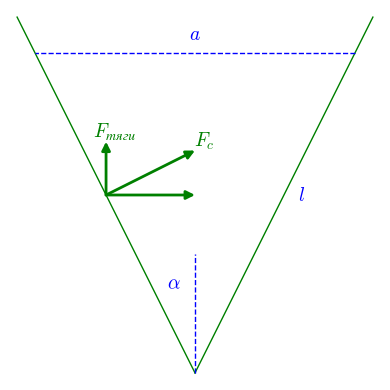
\includegraphics[width=0.48\textwidth]{Antipins_angle_ru.png}
\caption{}{Уголок Антипина}
\end{center}
\label{fig:Antipins_angle}
\end{wrapfigure}

    \section{Приложение D. Вывод формулы тяги сот на основе формулы Антипина
для тяги металлического
уголка}\label{ux43fux440ux438ux43bux43eux436ux435ux43dux438ux435-d.-ux432ux44bux432ux43eux434-ux444ux43eux440ux43cux443ux43bux44b-ux442ux44fux433ux438-ux441ux43eux442-ux43dux430-ux43eux441ux43dux43eux432ux435-ux444ux43eux440ux43cux443ux43bux44b-ux430ux43dux442ux438ux43fux438ux43dux430-ux434ux43bux44f-ux442ux44fux433ux438-ux43cux435ux442ux430ux43bux43bux438ux447ux435ux441ux43aux43eux433ux43e-ux443ux433ux43eux43bux43aux430}

    Антипин \cite{Antipin2012} приводит оценочный расчёт силы тяги «уголка»
при помощи формулы Казимира, «при самых общих и естественных
приближениях, известных, как PFA (Proximity Force Approximation), или
PAA (Pairwise Additive Approximation), способ расчёта
\cite{Intravaia2013}, \cite{Rodriguez2011}».

Энергия взаимодействия Казимира определяется выражением
\[\delta\,E/L^2 = \hbar\,c\frac{\pi^2}{4\,a^3}\left\{\frac{-4}{24\times30}\right\}\]

Сила Казимира
\[F_{c} = \hbar\,c\frac{-3\,\pi^2}{4\,a^4}\left\{\frac{-4}{24\times30}\right\}\]

Движущая сила металлического уголка

\[F_{тяги} = 2 \int F_{c} \, sin\, \alpha \,dS\]

\[dS = b\,dz\]

\[F_{тяги} = 2\, \frac{-3\,\pi^2\hbar c b}{4}\int\limits_{z_{min}}^{z_{max}} \left\{\frac{-4}{24\times30}\right\}\frac{sin\, \alpha}{\left(a\left(z\right)\right)^4}dz\]

делаем подстановку

\[a\left(z\right) = 2\,z\,tg\, \alpha\]

\[F_{тяги} = 2\, \frac{-3\,\pi^2\hbar c b}{4}\int\limits_{z_{min}}^{z_{max}} \left\{\frac{-4}{24\times30}\right\}\frac{sin\, \alpha}{\left(2\,z\,tg \alpha\right)^4}dz\]

\[F_{тяги} = 2\, \frac{-3\,\pi^2\hbar c b}{4} \frac{sin\, \alpha}{\left(2\,tg\, \alpha\right)^4} \int\limits_{z_{min}}^{z_{max}} \left\{\frac{-4}{24\times30}\right\} \frac{dz}{z^4}\]

\[F_{тяги} = -2\cdot3\, \frac{\pi^2\hbar c b}{240} \frac{sin\, \alpha}{\left(2\,tg\, \alpha\right)^4} \left(\frac{1}{z^3}\right)\Bigg\rvert_{\,z_{min}}^{\,z_{max}} \]

    Можно сделать подстановку \[z = l\, cos\, \alpha\]

\[F_{тяги} = -2\cdot3\, \frac{\pi^2\hbar c b}{240} \frac{sin\, \alpha}{2^4\left(tg\,\alpha\right)^4\left(cos\, \alpha\right)^3} \left(\frac{1}{l^3}\right)\Bigg\rvert_{\,l_{min}}^{\,l_{max}} \]

\[F_{тяги} = -2\cdot3\, \frac{\pi^2\hbar c b}{240} \frac{cos\, \alpha}{2^4\left(sin\, \alpha\right)^4} \left(\frac{1}{l^3}\right)\Bigg\rvert_{\,l_{min}}^{\,l_{max}} \]

\[F_{тяги} = \frac{\pi^2\hbar c b}{640} \frac{cos\, \alpha}{\left(sin\, \alpha\right)^4} \left(\frac{1}{l_{min}^3} - \frac{1}{l_{max}^3}\right)\]

Таким образом получена формула тяги уголка исходя из длины его крыльев.

Антипин указывает, что величина \(l_{min}\) ограничена снизу уровнем
«обрезания», который определяется технологически:

\begin{itemize}
\item
  точностью изготовления пластин (их шероховатостью, степенью
  плоскостности), а также
\item
  минимальной длиной волны фотонов, которые может эффективно отражать
  вещество, из которого изготовлен уголок (величиной \(k_m\)).
\end{itemize}

    Исследуя зависимость коэффициента в формуле тяги уголка, зависящего от
половинного угла раствора \(\alpha\) можно видеть, что при заданной
длине крыльев уголка выгоднее делать минимально возможный угол раствора.
Однако для целей настоящей работы (исследование возможности получения
тяги с помощью наносот) важно заметить что для уголка с прямым углом
\(\alpha = {\pi}/{4}\) коэффициент
\(\left({cos\, \alpha}\right)\big/\left({\left(sin\, \alpha\right)^4}\right) = 2\sqrt{2}\).
Таким образом составляя из множества прямоугольных уголков конструкцию в
виде сот показывается, что тяга панели состоящей из прямоугольных сот не
нулевая.

Действительно, прямоугольную соту с размером ячейки \(b \times b\) и с
такой же самой высотой ребра равной \(b = l_{max}\) можно представить
себе как комбинацию четырёх уголков с половинным углом раствора равным
\(\alpha = {\pi}/{4}\). Тягу каждого уголка

\[F_{тяги} = - \frac{\pi^2\hbar c l_{max}}{640} 2\sqrt{2} \left(\frac{1}{l_{min}^3} - \frac{1}{l_{max}^3}\right)\]

направленную вдоль биссектрисы каждого угла нужно умножить на
\(sin\left({\pi}/{4}\right)={\sqrt{2}}\big/{2}\) и при умножении на 4
тяга одной квадратной "распечатанной" соты будет равна

\[F_{тяги} = - \frac{\pi^2\hbar c b}{640} 2\sqrt{2}\cdot4\,\frac{\sqrt{2}}{2} \left(\frac{1}{l_{min}^3} - \frac{1}{b^3}\right)\]

\[F_{тяги} = - \frac{\pi^2\hbar c b}{640} 2\cdot4\,\left(\frac{1}{l_{min}^3} - \frac{1}{b^3}\right)\]

\[F_{тяги} = - \frac{\pi^2\hbar c b}{80} \left(\frac{1}{l_{min}^3} - \frac{1}{b^3}\right)\]

Итак, формула для удельной тяги сот, полученная с помощью метода PFA
(Proximity Force Approximation), или PAA (Pairwise Additive
Approximation)

\[\frac{F_{тяги}}{S} = - \frac{\pi^2\hbar c}{80\, b} \left(\frac{1}{l_{min}^3} - \frac{1}{b^3}\right)\]

в какой-то степени похожа на формулу величины двумерного эффекта
Казимира на сотах, произведённую в первой части данной работы: по
меньшей мере значением показатель степени в знаменателе совпадает.

\[\delta\,\frac{E}{V} \approx R\left(b k_m\right)\,\frac{\hbar\,c\,\pi}{b^4}\]

Здесь нужно отметить, что данная формула получена без учета конечности
высоты ребра сот (иными словами в приближении бесконечной высоты ребер),
в отличие от PFA варианта формулы для которого высота ребра принята
равной ширине ячейки.

Приблизительное соответствие этих формул говорит о том эффект должен
наблюдаться также и при конечной высоте ребер, хотя зависимость эффекта
от этой высоты может быть объектом дальнейших исследований.

С помощью панели из остроугольных уголков можно теоретически добиваться
бОльшей величины тяги, но технологически производство панелей из сот
представляется более простым, чем производство панелей из V-образных
уголков

    \begin{thebibliography}{99}

\bibitem{Casimir1948}
\textit{Casimir, H. B. G. (1948). On the attraction between two perfectly conducting plates. Proc. K. Ned. Akad. Wet. B 51, 793–5.
https://www.dwc.knaw.nl/DL/publications/PU00018547.pdf}

\bibitem{Boyer1968}
\textit{Boyer, T. H. (1968). Quantum electromagnetic zero-point energy of a conducting spherical shell and Casimir model for a charged particle. Phys. Rev. 174, 1764–76.}

\bibitem{Antipin2012}
\textit{Antipin A. V. (2012). RU 2 610 018 C2. Method for propulsion of bodies by Casimir effect and/or its analogue.}

\bibitem{Bikyalis1968}
\textit{A.Bikyalis (1968). Euler-Maclaurin summation formula for a function of many variables.  Lietuvos matematikos rinkinys. Литовский математический сборник. p.681
https://www.journals.vu.lt/LMJ/article/view/20600/19701}

\bibitem{Tuo2019}
\textit{Tuo Qu, Fang Liu, Yuechai Lin, Yidong Huang, "Metal nano-honeycomb fabricated by colloidal assembly and femtosecond-laser annealing," Proc. SPIE 10841, 9th International Symposium on Advanced Optical Manufacturing and Testing Technologies: Meta-Surface-Wave and Planar Optics, 108410A (30 January 2019); https://doi.org/10.1117/12.2508593}

\bibitem{Hrvoje2016}
\textit{Nikolic, Hrvoje (2016). "Proof that Casimir force does not originate from vacuum energy". Physics Letters B. 761: 197–202. arXiv:1605.04143. Bibcode:2016PhLB..761..197N. doi:10.1016/j.physletb.2016.08.036. S2CID 119265677.}

\bibitem{Intravaia2013}
\textit{F. Intravaia et al., Strong Casimir force reduction through metallic surface nanostructuring // Nature Comm, art. 2515, 4 (Sep. 2013) pp. 1-20}

\bibitem{Rodriguez2011}
\textit{A.W. Rodriguez, F. Capasso, S.G. Johnson, The Casimir effect in microstructured geometries // Nature Photonics, V.5, (Apr. 2011), p.211-221}

\end{thebibliography}


    % Add a bibliography block to the postdoc
    
    
    
\end{document}
